\documentclass[12pt,letterpaper,oneside]{book}
\usepackage{../../afitStyleFiles/afitThesis}
\usepackage[nolist]{acronym}
\usepackage{todo}
\usepackage{tabu}
\usepackage{makecell}
\renewcommand\theadfont{\bfseries}
\graphicspath{{../../Figures/}}
%% myFigures.tex
% A common file to store all figure definitions
%
% In preparing your thesis, one of the first things you should do is
% organize your figures.  Then, one of the last things you'll do is
% reorder your figures so they display where you want them to in the
% text.  Organizing figure definitions in a common files helps:
%
%   1. Write new figures using earlier examples.
%
%   2.  Isolate code and minimize the risk of introducing bugs in the
%   final editing process.  Trust me, moving around just one line of
%   code is easier.
%
%   3.  Reuse figures in other papers.  <=== the best reason!
%
% Note command names can not include numbers and special characters.
%
% To make the file more searchable, use naming conventions that map
% the graphics filename labSetup.jpg to the command name \figlabSetup to the
% figure label fig:labSetup.
% 

\newcommand{\figMpduFormat}{
	\begin{figure}[H]
		\begin{center}
			\makebox[\textwidth][c]{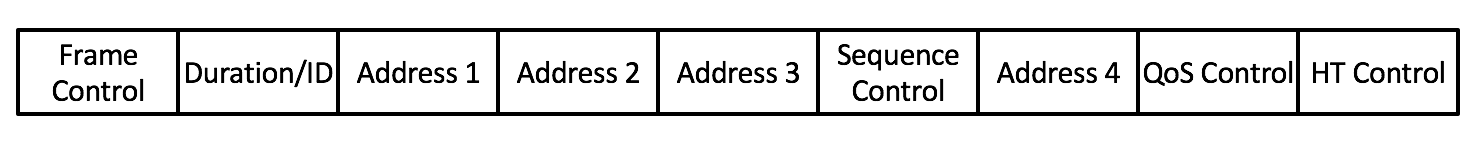
\includegraphics[width=\linewidth]{macHeader}}
			\caption{\ac{MPDU} format when using \ac{WPA}-2 \cite{802.11}}
			\label{fig:MpduFormat}
		\end{center}
		\vspace{-0.2 in}
	\end{figure}
}

\newcommand{\figMacHeader}{
	\begin{figure}[H]
		\begin{center}
			\makebox[\textwidth][c]{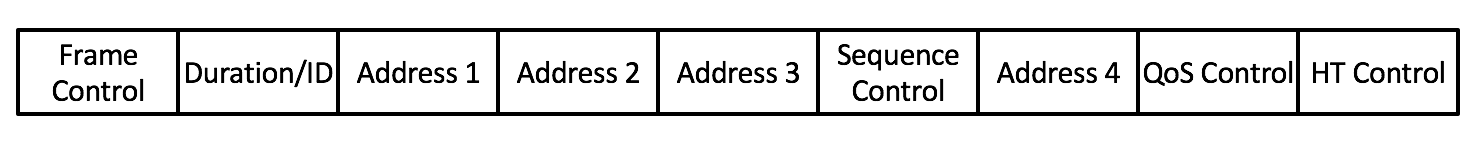
\includegraphics[width=\linewidth]{macHeader}}
			\caption{\ac{MAC} Header Frame Format \cite{802.11}}
			\label{fig:MacHeader}
		\end{center}
		\vspace{-0.2 in}
	\end{figure}
}

\newcommand{\figArchitecture}{\begin{figure}[H]
	\begin{center}
		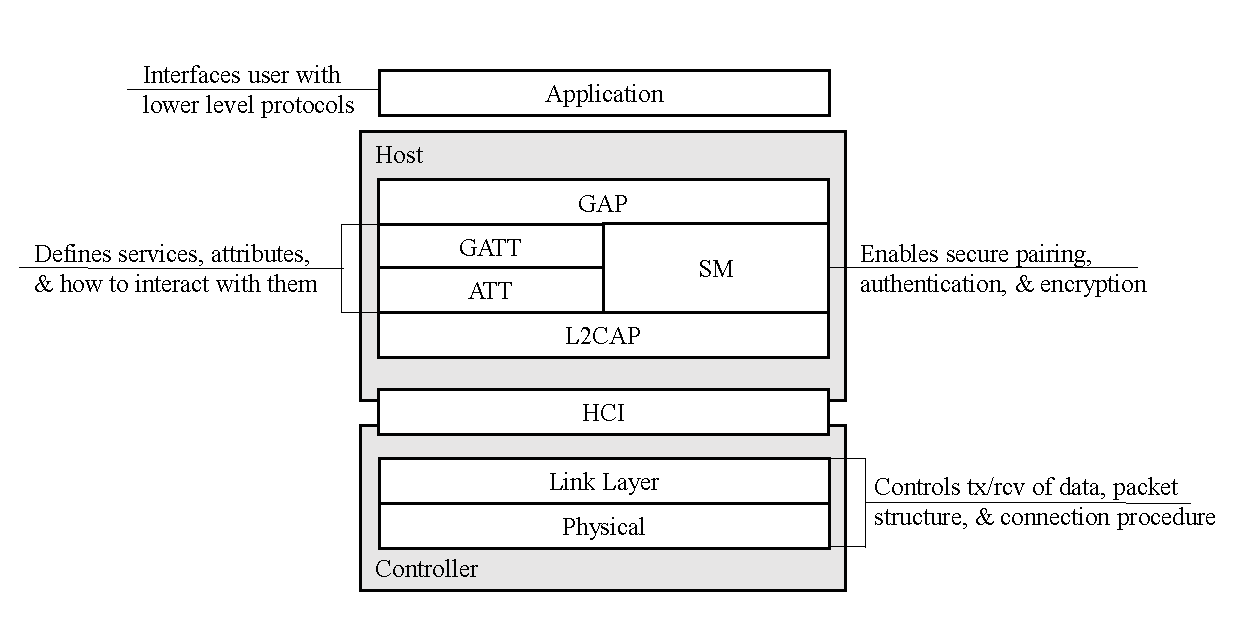
\includegraphics[width=4in]{architecture}
		\caption{The Bluetooth Low Energy Architecture}
		\label{fig:Architecture}
	\end{center}
	\vspace{-0.2 in}
\end{figure}
}

\newcommand{\figConnection}{\begin{figure}[H]
	\begin{center}
		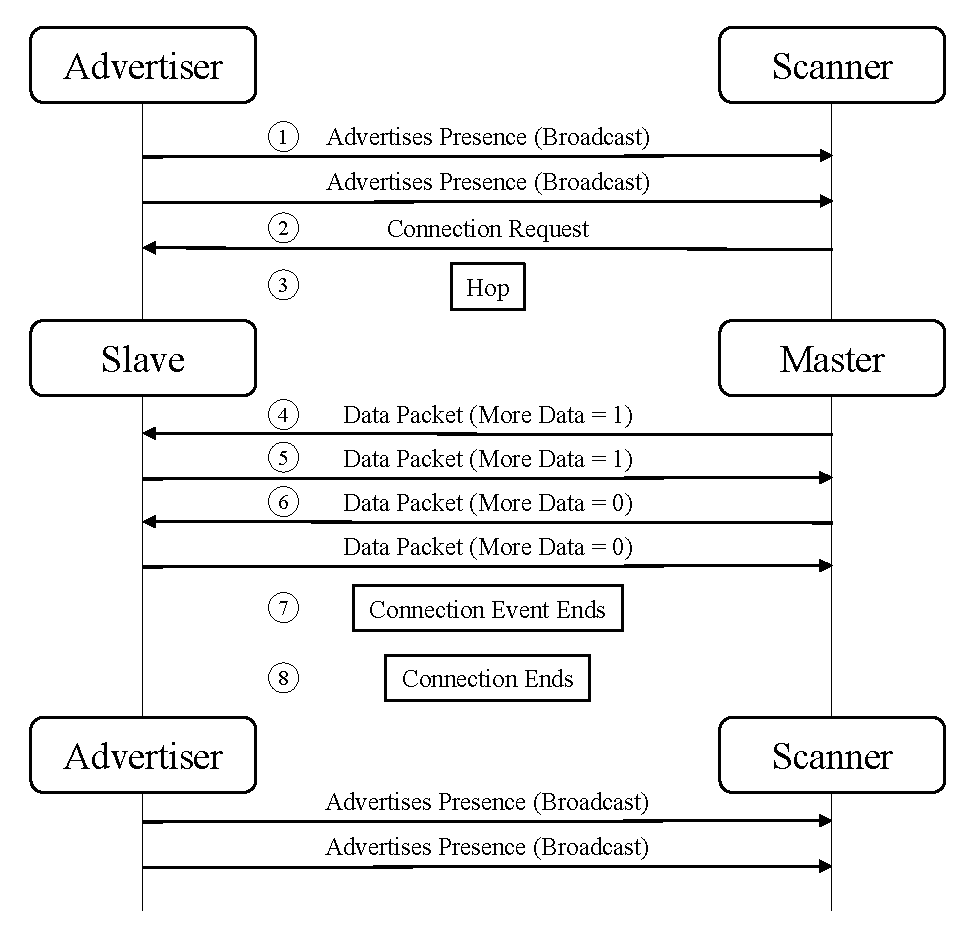
\includegraphics[width=4in]{connectionProcess}
		\caption{The \ac{BLE} Connection Process}
		\label{fig:Connection}
	\end{center}
	\vspace{-0.2 in}
\end{figure}
}

\newcommand{\figScanning}{\begin{figure}[H]
		\begin{center}
			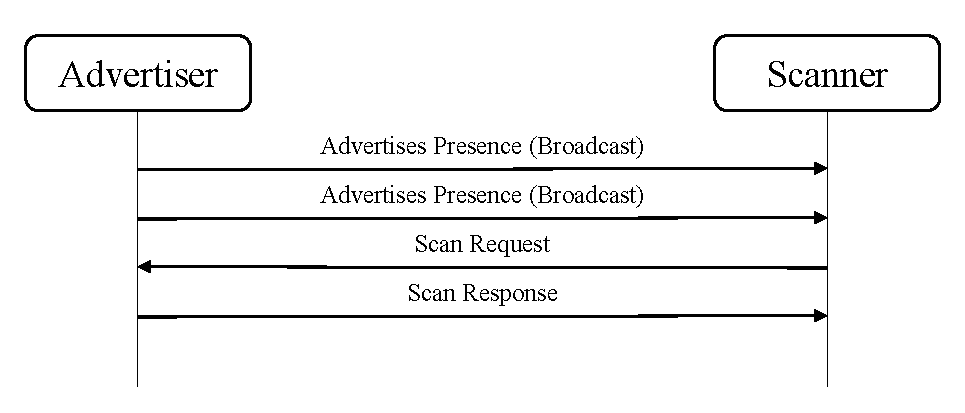
\includegraphics[width=4in]{activeScanning}
			\caption{Active Scanning Process}
			\label{fig:Scanning}
		\end{center}
		\vspace{-0.2 in}
	\end{figure}
}

\newcommand{\figChannel}{
	\begin{figure}[H]
		\begin{center}
			\includegraphics[width=5in]{channelMap}
			\caption{Bluetooth Low Energy channel mapping; darker channels represent advertisement channels}
			\label{fig:Channel}
		\end{center}
		\vspace{-0.2 in}
	\end{figure}
}

\newcommand{\figAccessPoint}{
	\begin{figure}[H]
		\begin{center}
			\makebox[\textwidth][c]{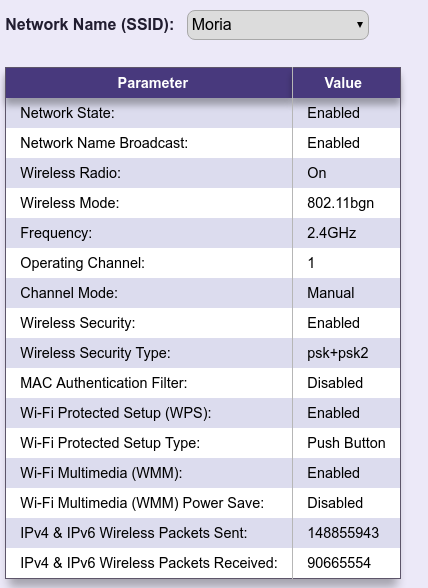
\includegraphics[width=2.5in]{accessPoint}}
			\caption{Prancing Pony Access Point Settings}
			\label{fig:AccessPoint}
		\end{center}
		\vspace{-0.2 in}
	\end{figure}
}

\newcommand{\figSystemDiagram}{
	\begin{figure}[h!]
		\begin{center}
			\centering
			\makebox[\textwidth][c]{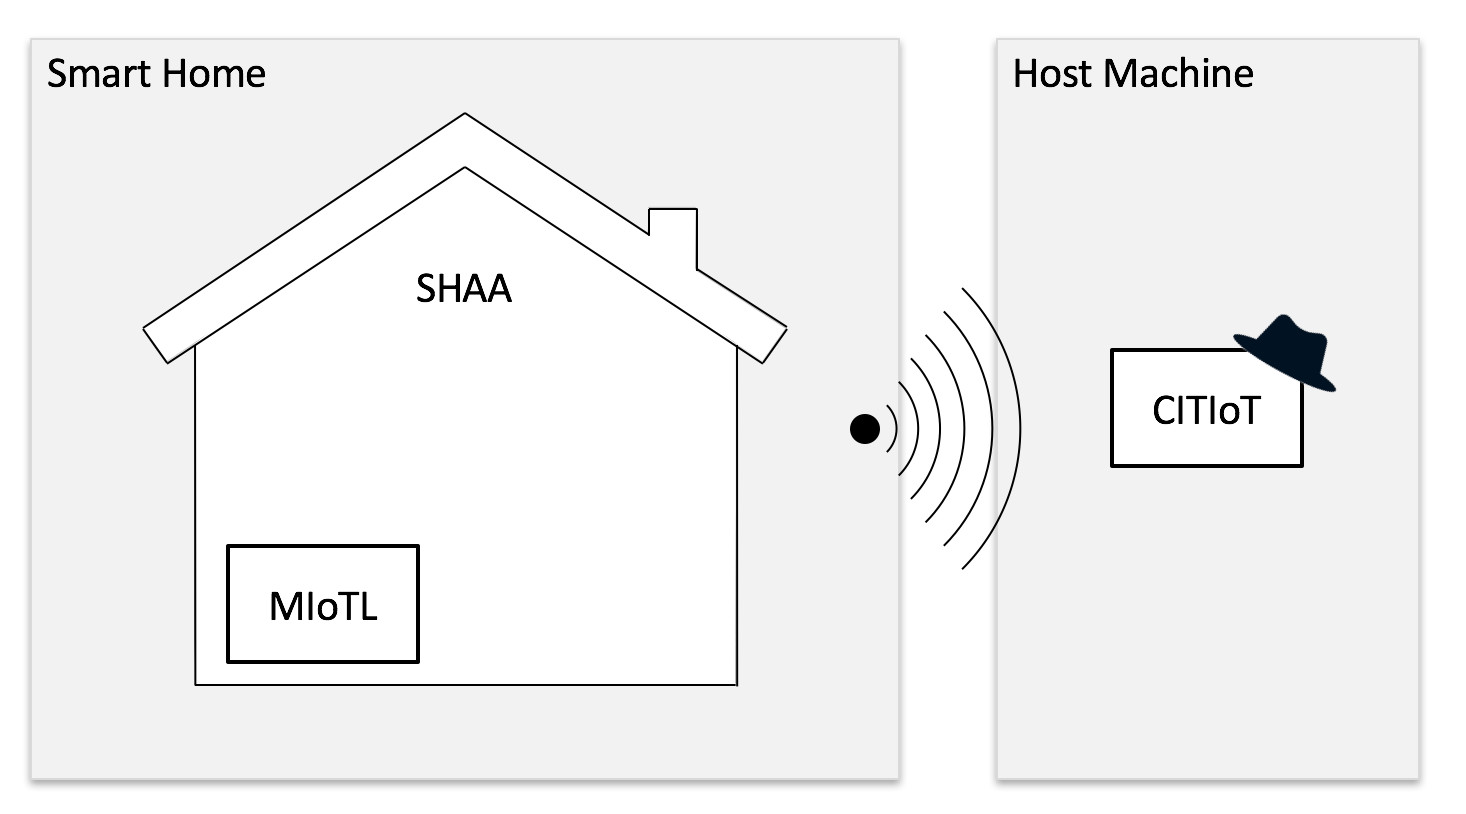
\includegraphics[width=4in]{systemDiagram}}
			\caption{Overall system diagram}
			\label{fig:SystemDiagram}
		\end{center}
		\vspace{-0.2 in}
	\end{figure}
}

\newcommand{\figShaaDiagram}{
	\begin{figure*}[h!]
		\begin{center}
			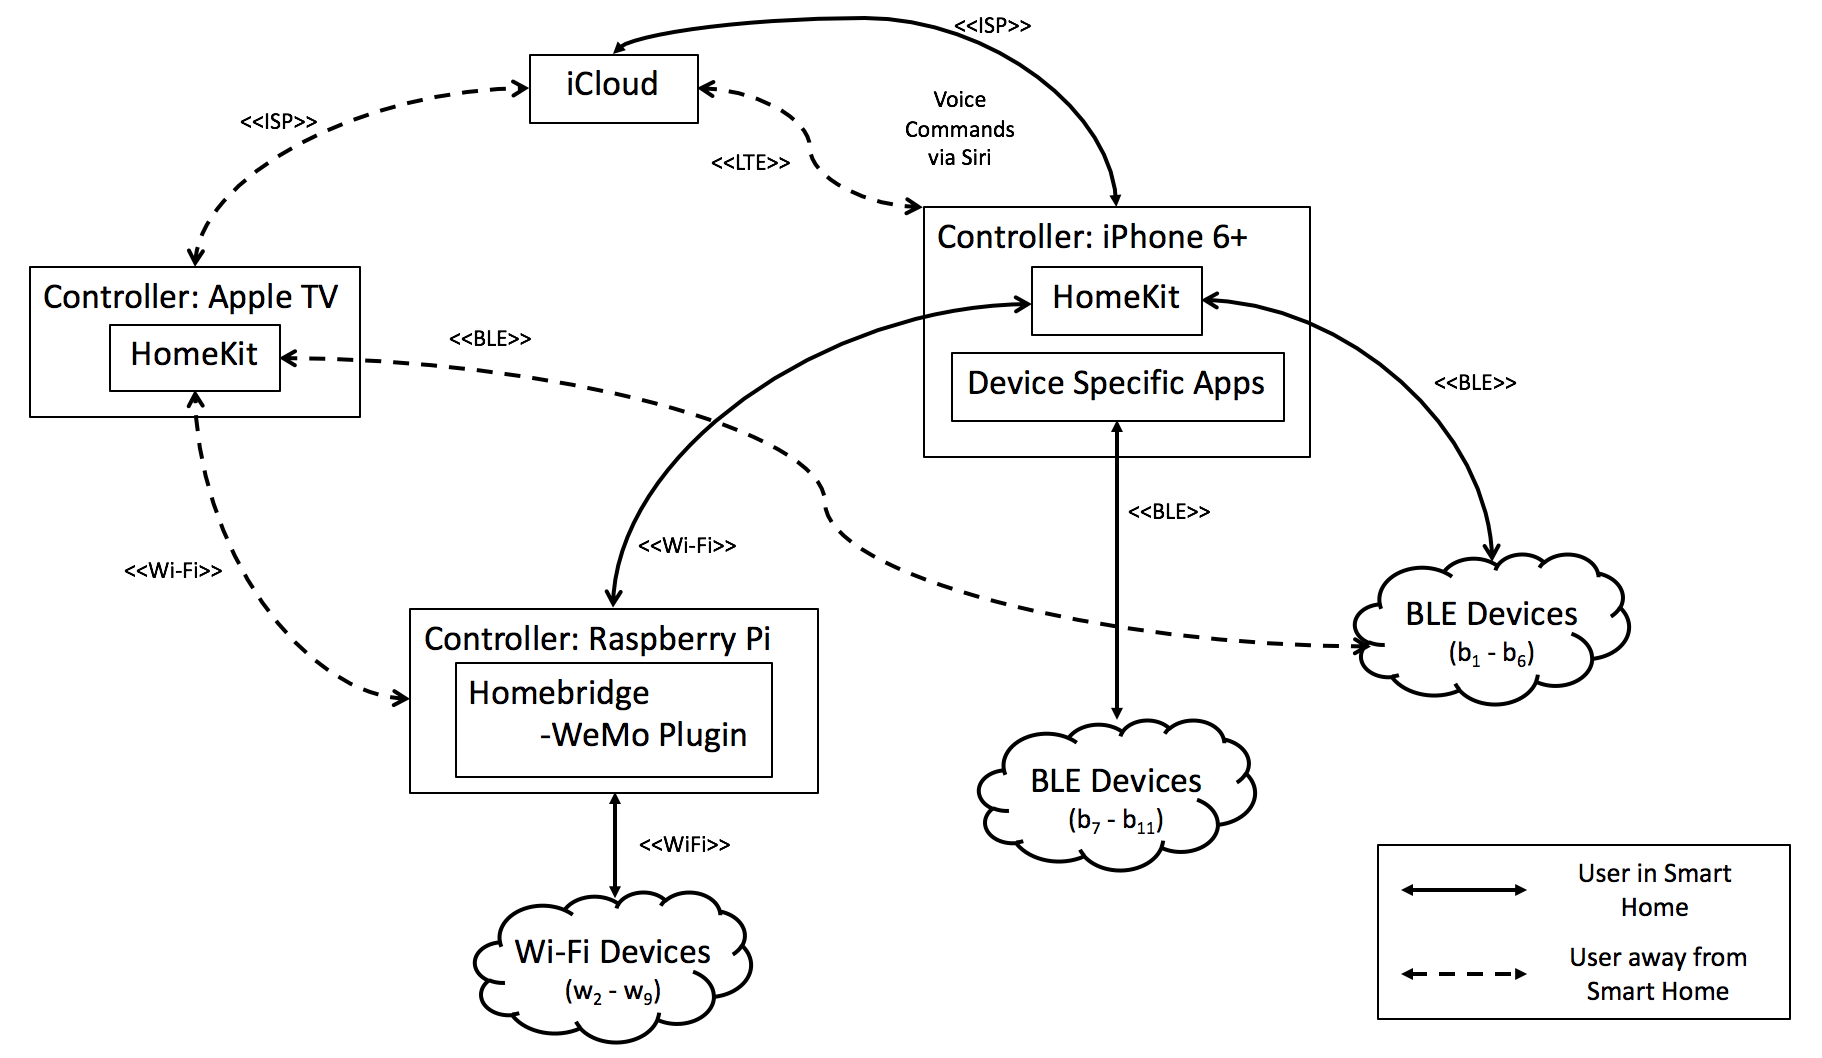
\includegraphics[width=\linewidth]{shaaDiagram}
			\caption{Diagram of SHAA components}
			\label{fig:ShaaDiagram}
		\end{center}
		\vspace{-0.2 in}
	\end{figure*}
}

\newcommand{\figCitiotDiagram}{
	\begin{figure*}[h!]
		\begin{center}
			\makebox[\textwidth][c]{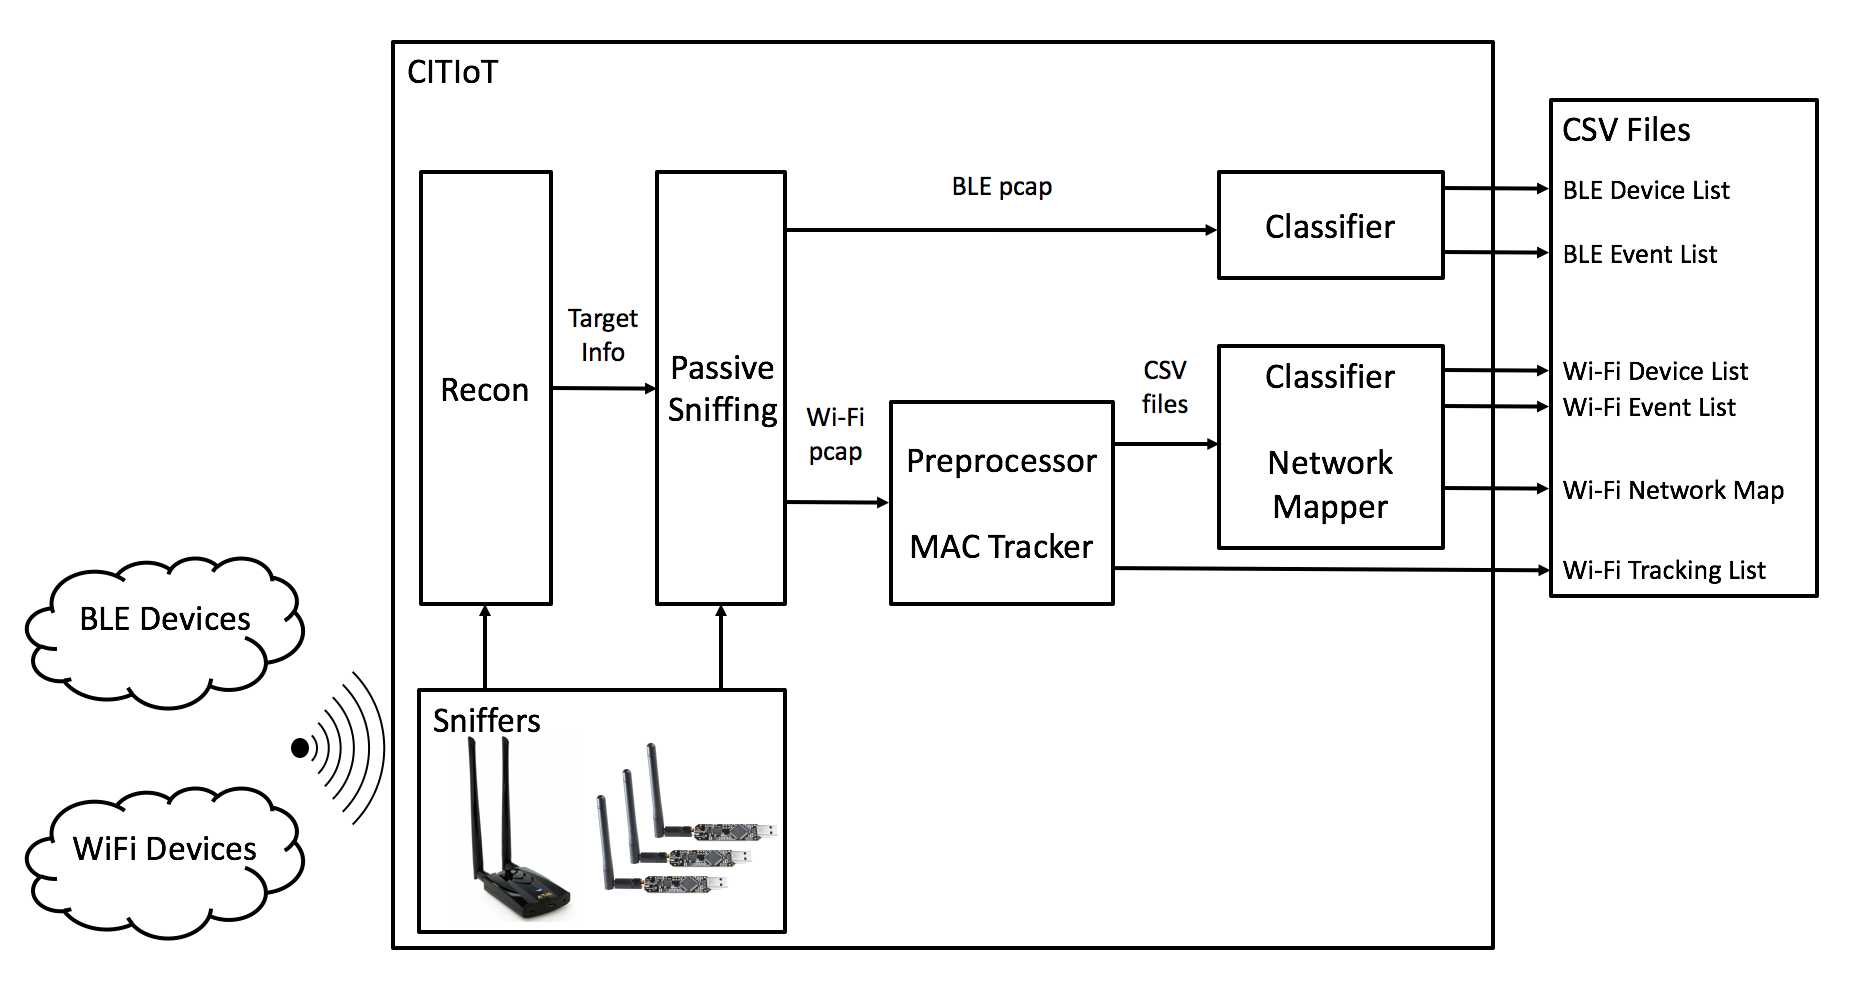
\includegraphics[width=\linewidth]{citiotDiagram}}
			\caption{Diagram of CITIoT tool components and interactions}
			\label{fig:CitiotDiagram}
		\end{center}
		\vspace{-0.2 in}
	\end{figure*}
}

\newcommand{\figReconScan}{
	\begin{figure*}[h!]
		\begin{center}
			\makebox[\textwidth][c]{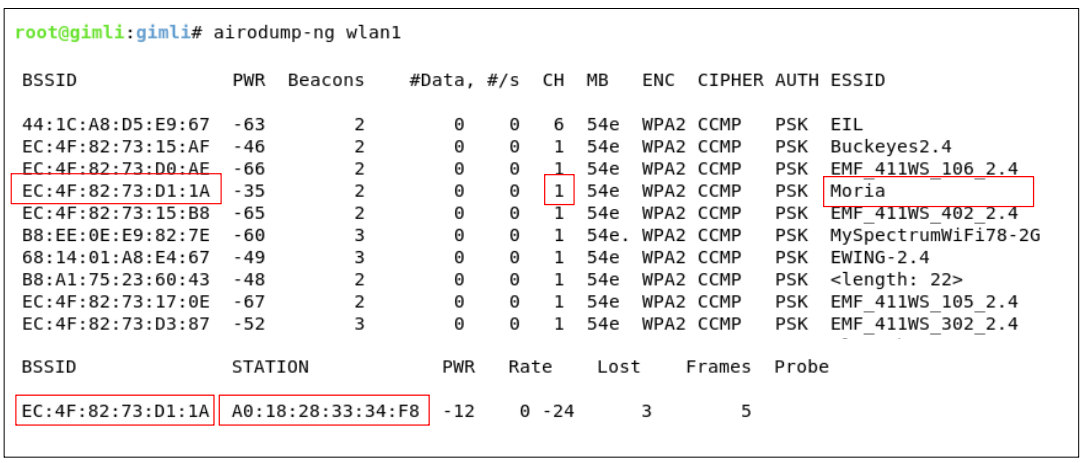
\includegraphics[width=\linewidth]{reconScan}}
			\caption{Command and results to accomplish a scan of Wi-Fi devices and associated \ac{AP}s}
			\label{fig:ReconScan}
		\end{center}
		\vspace{-0.2 in}
	\end{figure*}
}

\newcommand{\figScanDevices}{
	\begin{figure}[H]
		\begin{center}
			\makebox[\textwidth][c]{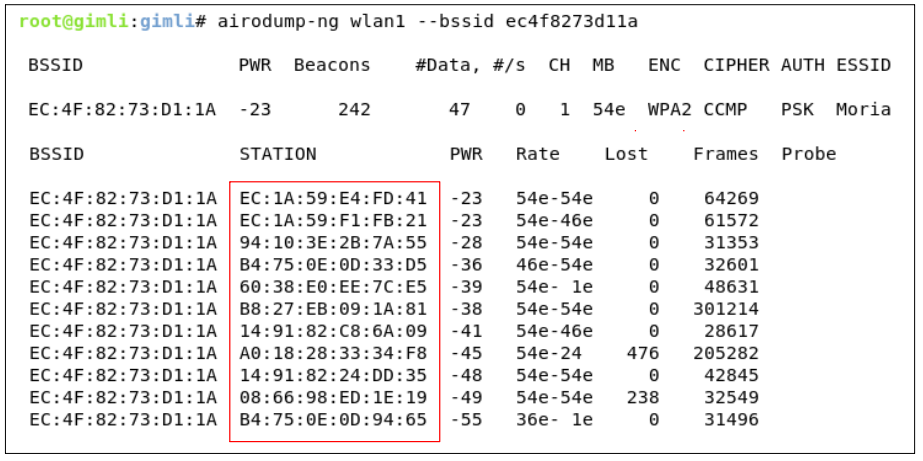
\includegraphics[width=\linewidth]{scanDevices}}
			\caption{Command and results to scan for devices connected to the target \ac{AP}}
			\label{fig:ScanDevices}
		\end{center}
		\vspace{-0.2 in}
	\end{figure}
}

\newcommand{\figOuiLookup}{
	\begin{figure}[H]
		\begin{center}
			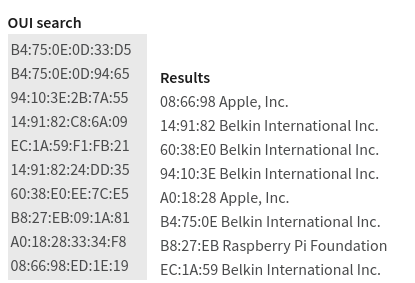
\includegraphics[width=3in]{ouiLookup}
			\caption{Wi-Fi MAC OUI search and results}
			\label{fig:OuiLookup}
		\end{center}
		\vspace{-0.2 in}
	\end{figure}
}

\newcommand{\figBleDeviceScan}{
	\begin{figure}[H]
		\begin{center}
			\makebox[\textwidth][c]{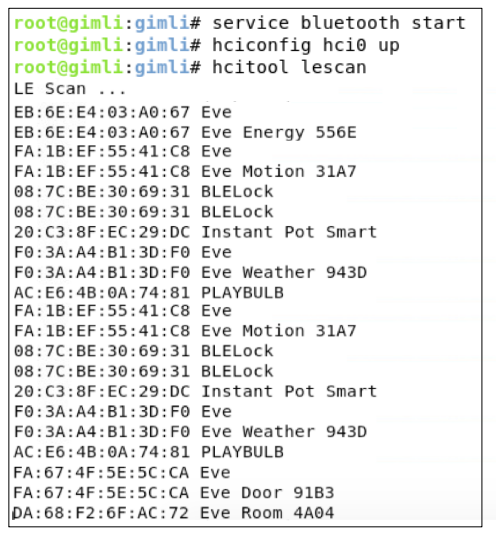
\includegraphics[width=3.5in]{bleDeviceScan}}
			\caption{Command and results to scan for \ac{BLE} devices within the smart home}
			\label{fig:BleDeviceScan}
		\end{center}
		\vspace{-0.2 in}
	\end{figure}
}

\newcommand{\figMonitorMode}{
	\begin{figure}[H]
		\begin{center}
			\makebox[\textwidth][c]{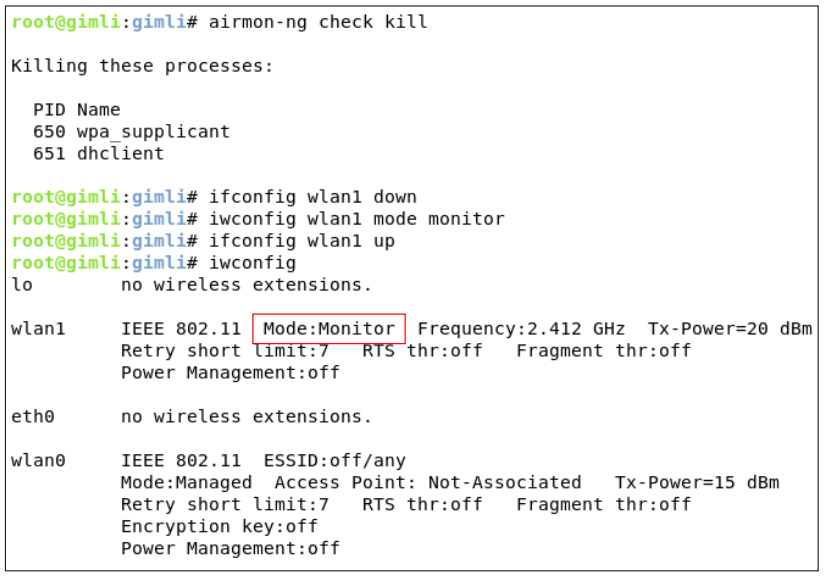
\includegraphics[width=\linewidth]{monitorMode}}
			\caption{Commands used to set Wi-Fi interface to monitor mode}
			\label{fig:MonitorMode}
		\end{center}
		\vspace{-0.2 in}
	\end{figure}
}

\newcommand{\figWifiCaptCmd}{
	\begin{figure}[H]
		\begin{center}
			\makebox[\textwidth][c]{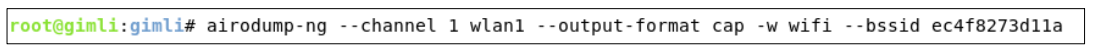
\includegraphics[height=.75cm]{wifiCaptCmd}}
			\caption{Command and options used to capture Wi-Fi traffic}
			\label{fig:WifiCaptCmd}
		\end{center}
		\vspace{-0.2 in}
	\end{figure}
}

\newcommand{\figBleCaptCmd}{
	\begin{figure}[H]
		\begin{center}
			\makebox[\textwidth][c]{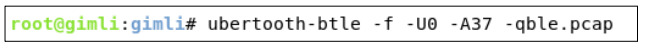
\includegraphics[height=.75cm]{bleCaptCmd}}
			\caption{Example command and options used to capture \ac{BLE} traffic}
			\label{fig:BleCaptCmd}
		\end{center}
		\vspace{-0.2 in}
	\end{figure}
}

\newcommand{\figCorruptTimePacket}{
	\begin{figure}[H]
		\begin{center}
			\makebox[\textwidth][c]{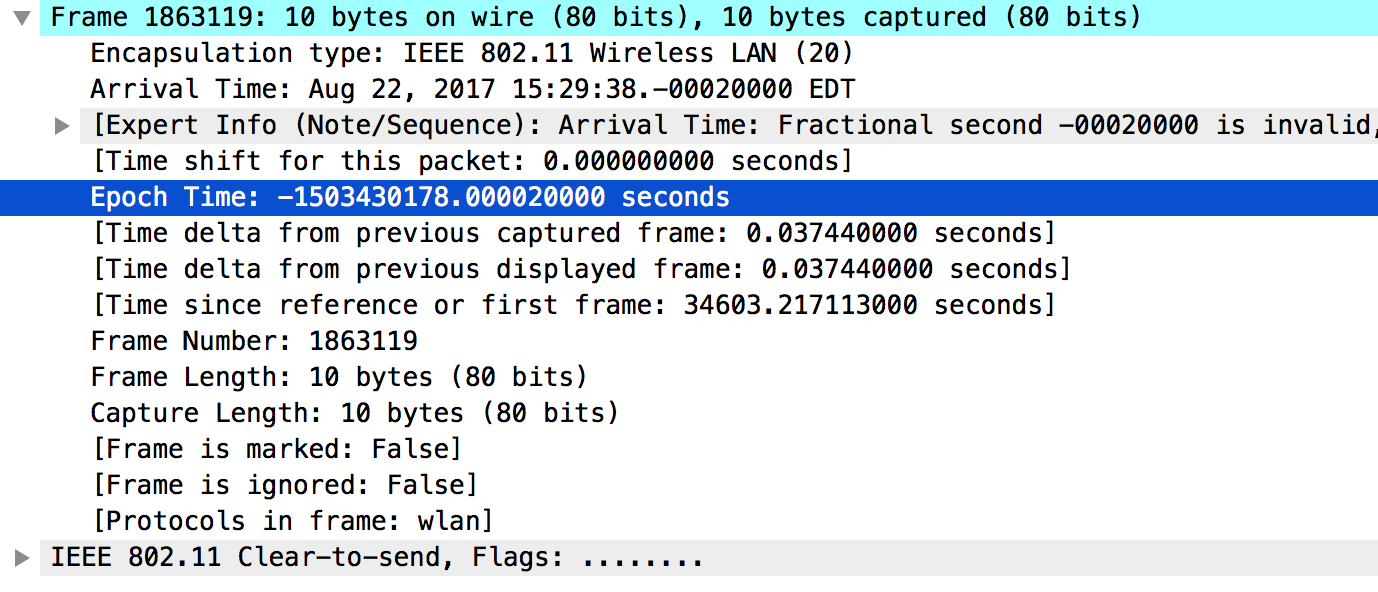
\includegraphics[width=\linewidth]{corruptTimePacket}}
			\caption{Encrypted packet used in \ac{MAC} tracker showing corrupted timestamp}
			\label{fig:CorruptTimePacket}
		\end{center}
		\vspace{-0.2 in}
	\end{figure}
}

\newcommand{\figWrongFrameNumber}{
	\begin{figure}[H]
		\begin{center}
			\makebox[\textwidth][c]{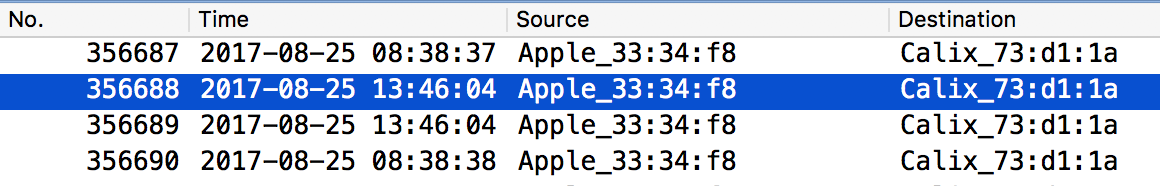
\includegraphics[width=\linewidth]{wrongFrameNumber}}
			\caption{Encrypted packets used in \ac{MAC} tracker showing sequential frame numbers but wrong times}
			\label{fig:WrongFrameNumber}
		\end{center}
		\vspace{-0.2 in}
	\end{figure}
}

\newcommand{\figTrainingToDevice}{
	\begin{figure}[H]
		\centering
		\begin{subfigure}{.485\textwidth}
			\centering
			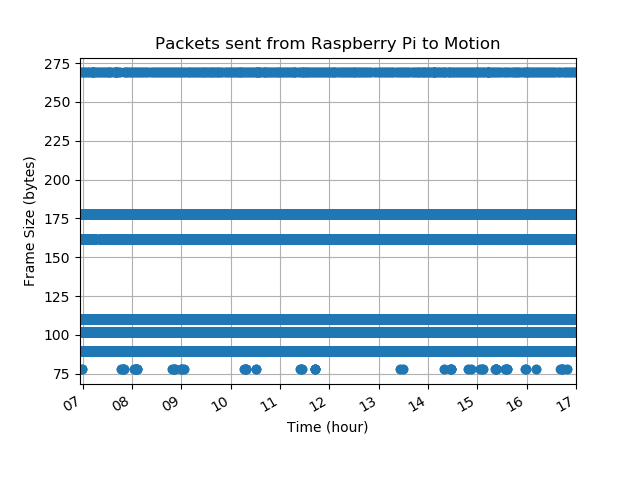
\includegraphics[width=\linewidth]{trngToMotion}
			\caption{}
		\end{subfigure}%
		\begin{subfigure}{.485\textwidth}
			\centering
			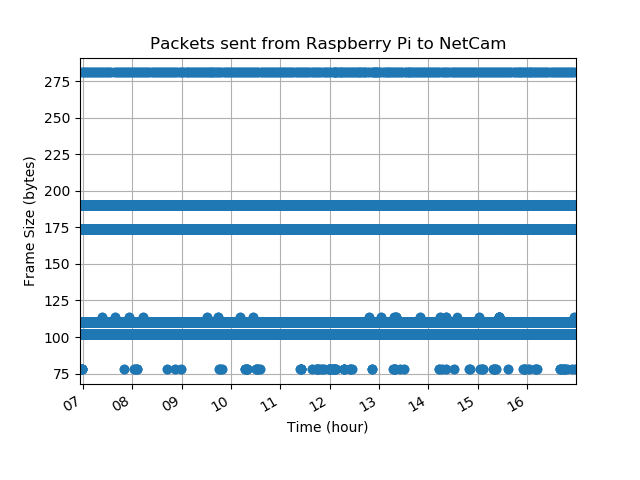
\includegraphics[width=\linewidth]{trngToNetcam}
			\caption{}
		\end{subfigure}
		\begin{subfigure}{.485\textwidth}
			\centering
			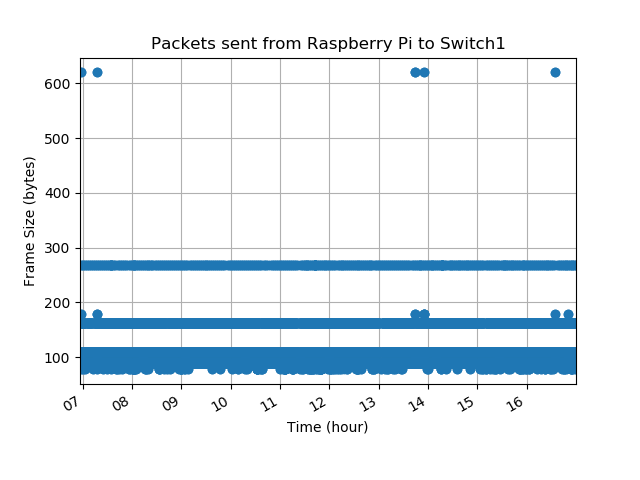
\includegraphics[width=\linewidth]{trngToSwitch1}
			\caption{}
		\end{subfigure}%
		\begin{subfigure}{.485\textwidth}
			\centering
			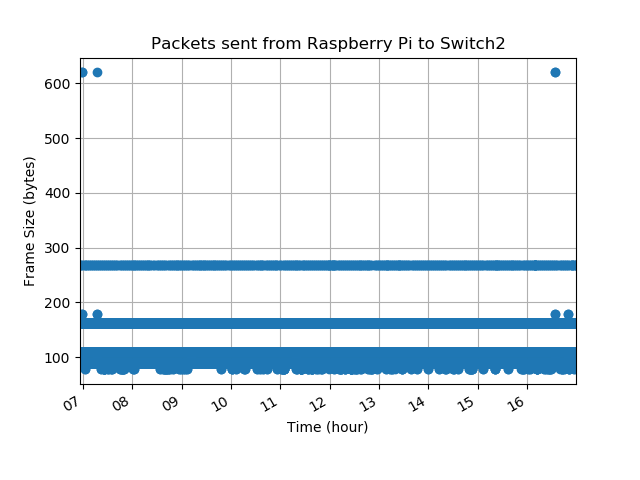
\includegraphics[width=\linewidth]{trngToSwitch2}
			\caption{}
		\end{subfigure}
		\begin{subfigure}{.485\textwidth}
			\centering
			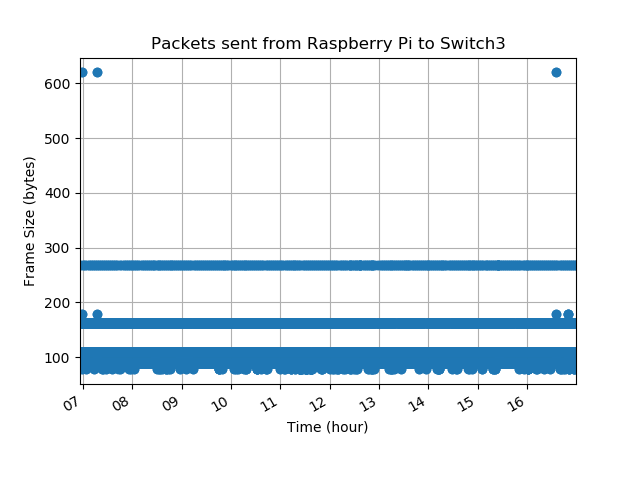
\includegraphics[width=\linewidth]{trngToSwitch3}
			\caption{}
		\end{subfigure}%
		\begin{subfigure}{.485\textwidth}
			\centering
			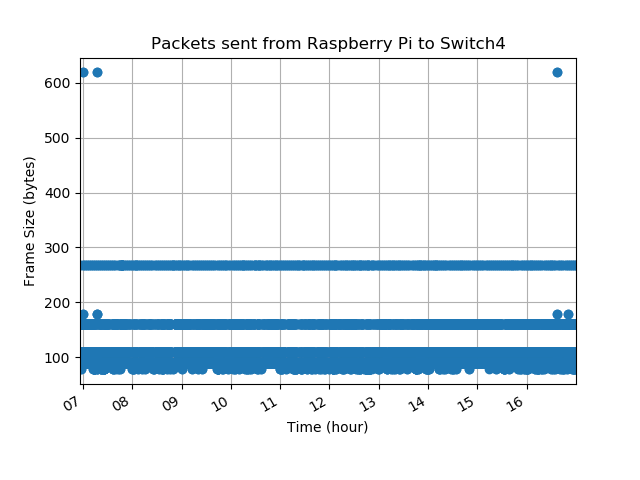
\includegraphics[width=\linewidth]{trngToSwitch4}
			\caption{}
		\end{subfigure}
		\begin{subfigure}{.485\textwidth}
			\centering
			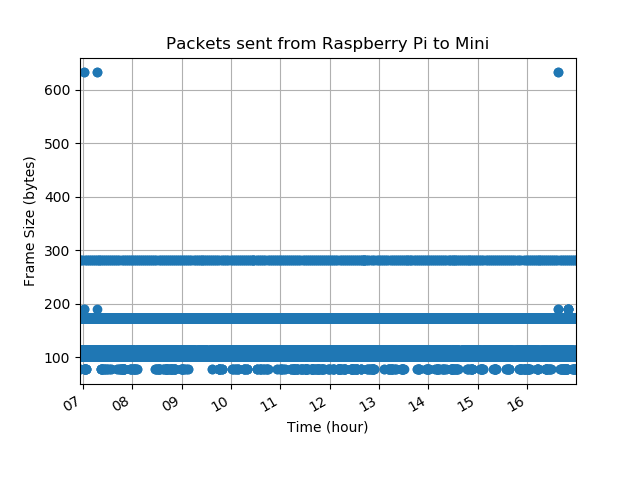
\includegraphics[width=\linewidth]{trngToMini}
			\caption{}
		\end{subfigure}%
		\begin{subfigure}{.485\textwidth}
			\centering
			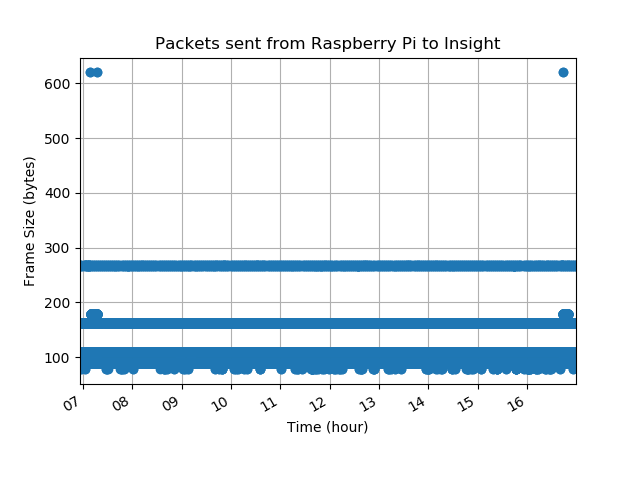
\includegraphics[width=\linewidth]{trngToInsight}
			\caption{}
		\end{subfigure}
		\caption{Training plots of packets sent from raspberry pi to device}
		\label{fig:TrainingToDevice}
	\end{figure}
}

\newcommand{\figTrainingFromDevice}{
	\begin{figure}[H]
		\centering
		\begin{subfigure}{.485\textwidth}
			\centering
			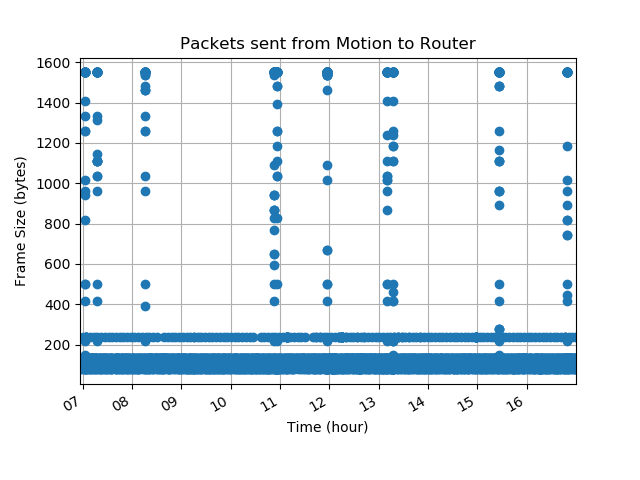
\includegraphics[width=\linewidth]{trngFromMotion}
			\caption{}
		\end{subfigure}%
		\begin{subfigure}{.485\textwidth}
			\centering
			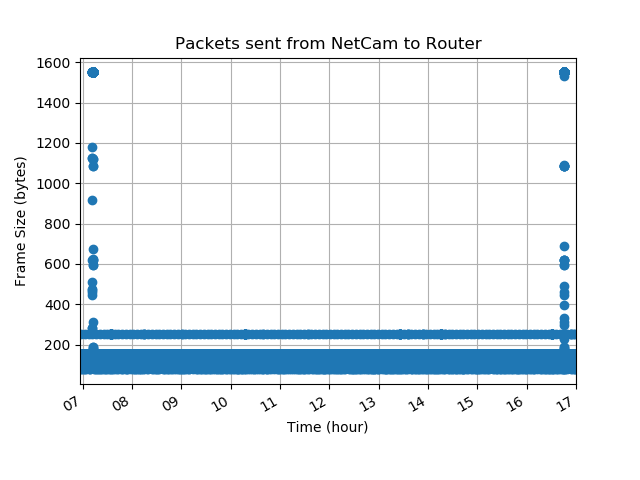
\includegraphics[width=\linewidth]{trngFromNetcam}
			\caption{}
		\end{subfigure}
		\begin{subfigure}{.485\textwidth}
			\centering
			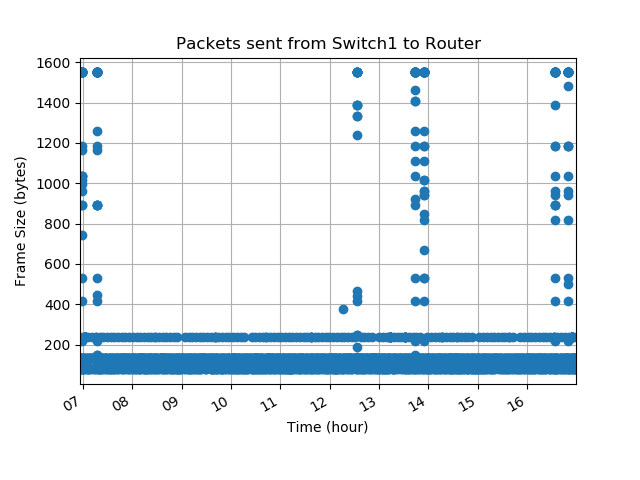
\includegraphics[width=\linewidth]{trngFromSwitch1}
			\caption{}
		\end{subfigure}%
		\begin{subfigure}{.485\textwidth}
			\centering
			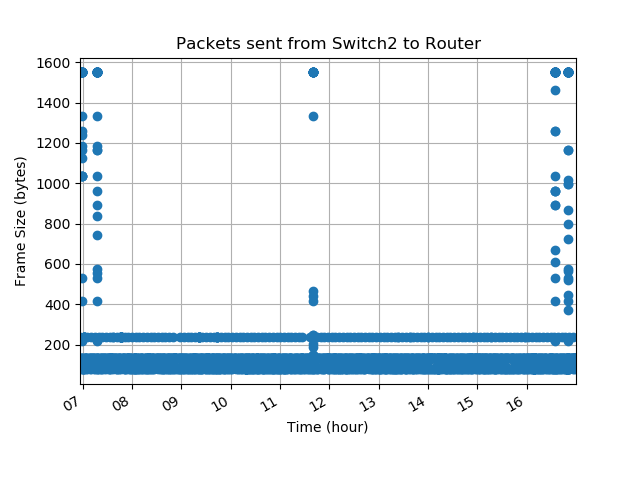
\includegraphics[width=\linewidth]{trngFromSwitch2}
			\caption{}
		\end{subfigure}
		\begin{subfigure}{.485\textwidth}
			\centering
			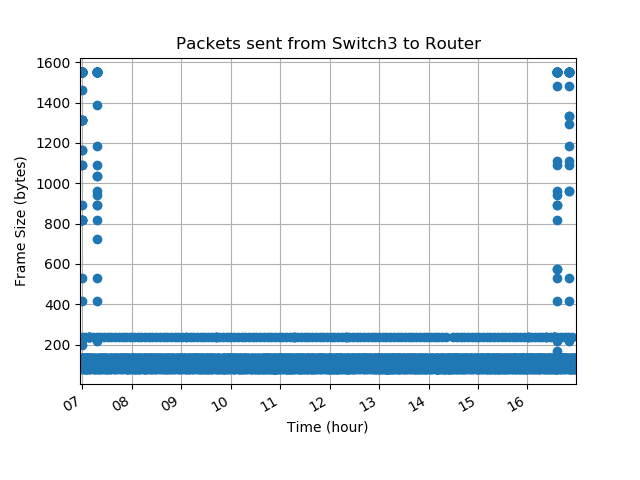
\includegraphics[width=\linewidth]{trngFromSwitch3}
			\caption{}
		\end{subfigure}%
		\begin{subfigure}{.485\textwidth}
			\centering
			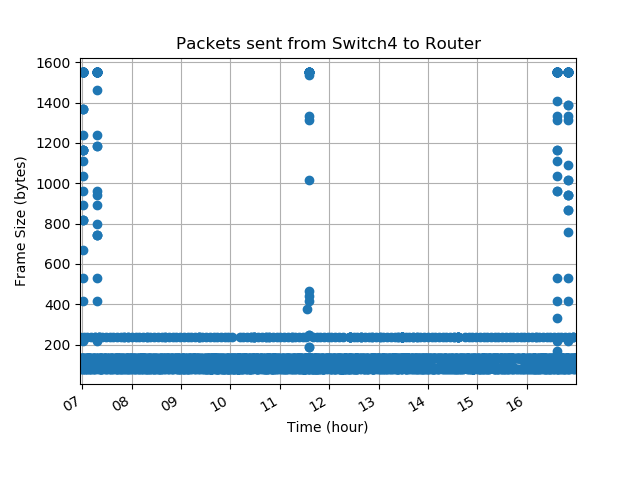
\includegraphics[width=\linewidth]{trngFromSwitch4}
			\caption{}
		\end{subfigure}
		\begin{subfigure}{.485\textwidth}
			\centering
			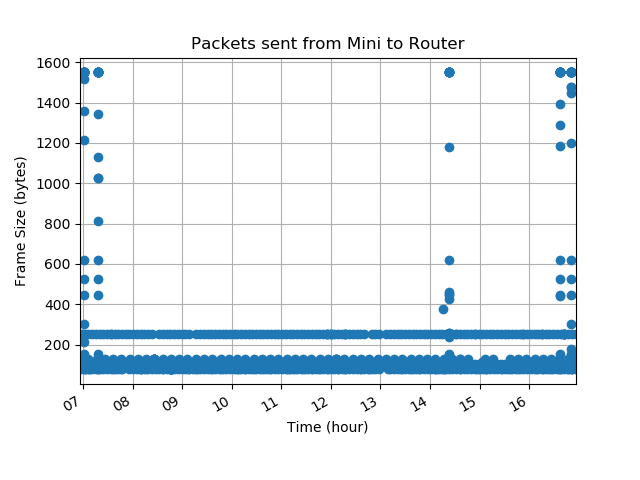
\includegraphics[width=\linewidth]{trngFromMini}
			\caption{}
		\end{subfigure}%
		\begin{subfigure}{.485\textwidth}
			\centering
			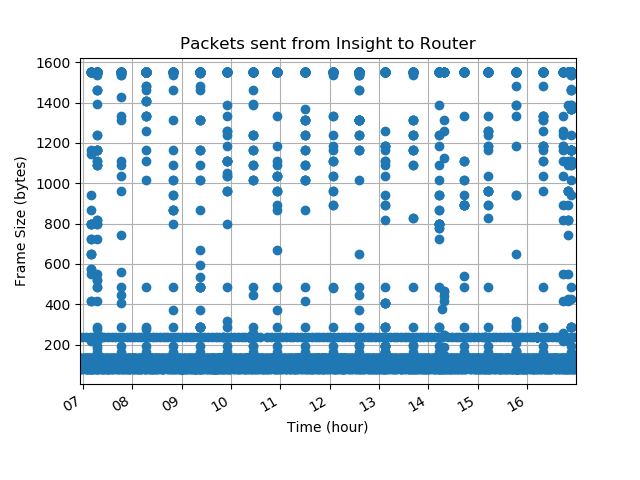
\includegraphics[width=\linewidth]{trngFromInsight}
			\caption{}
		\end{subfigure}
		\caption{Training plots of packets sent from device to the router}
		\label{fig:TrainingFromDevice}
	\end{figure}
}

\newcommand{\figClassificationToNetcam}{
	\begin{figure}[H]
		\begin{center}
			\makebox[\textwidth][c]{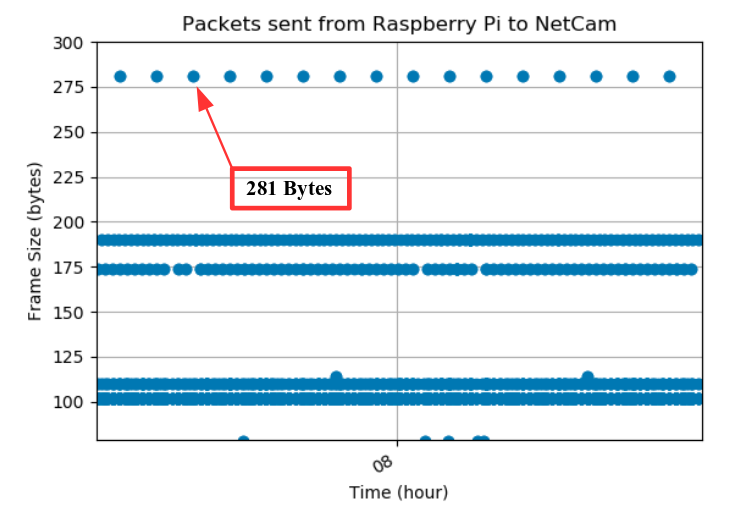
\includegraphics[width=5in]{classificationToNetcam}}
			\caption{Figure~\ref{fig:TrainingToDevice}(b) zoomed in on unique packet traffic used to classify camera devices}
			\label{fig:ClassificationToNetcam}
		\end{center}
		\vspace{-0.2 in}
	\end{figure}
}

\newcommand{\figClassificationToMotion}{
	\begin{figure}[H]
		\begin{center}
			\makebox[\textwidth][c]{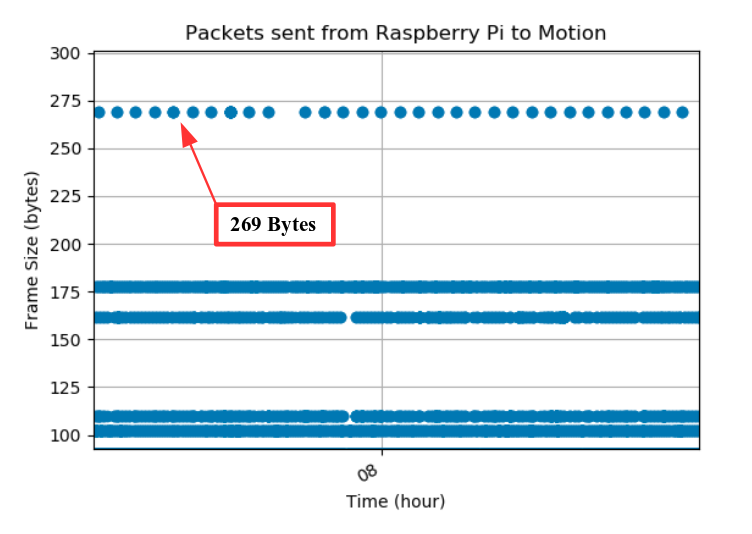
\includegraphics[width=5in]{classificationToMotion}}
			\caption{Figure~\ref{fig:TrainingToDevice}(a) zoomed in on unique packet traffic used to classify motion devices}
			\label{fig:ClassificationToMotion}
		\end{center}
		\vspace{-0.2 in}
	\end{figure}
}

\newcommand{\figClassificationToSwitch}{
	\begin{figure}[H]
		\begin{center}
			\makebox[\textwidth][c]{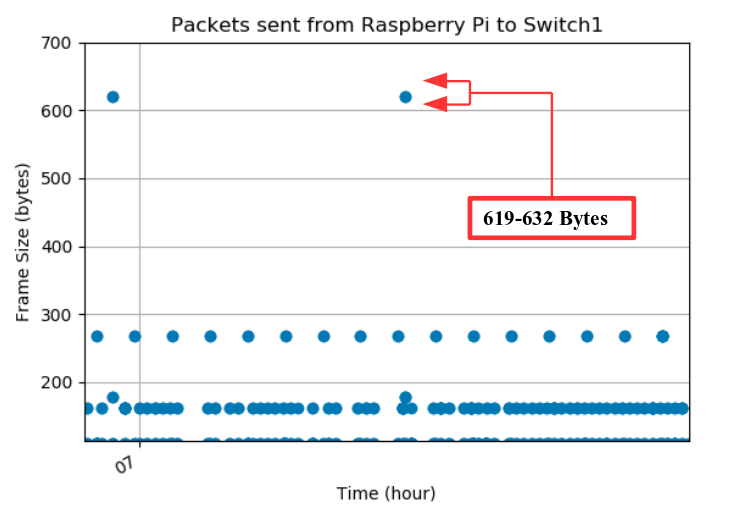
\includegraphics[width=5in]{classificationToSwitch}}
			\caption{Figure~\ref{fig:TrainingToDevice}(c) zoomed in on unique packet traffic used to classify outlet devices}
			\label{fig:ClassificationToSwitch}
		\end{center}
		\vspace{-0.2 in}
	\end{figure}
}

\newcommand{\figDeviceClassification}{
	\begin{figure}[H]
		\begin{center}
			\makebox[\textwidth][c]{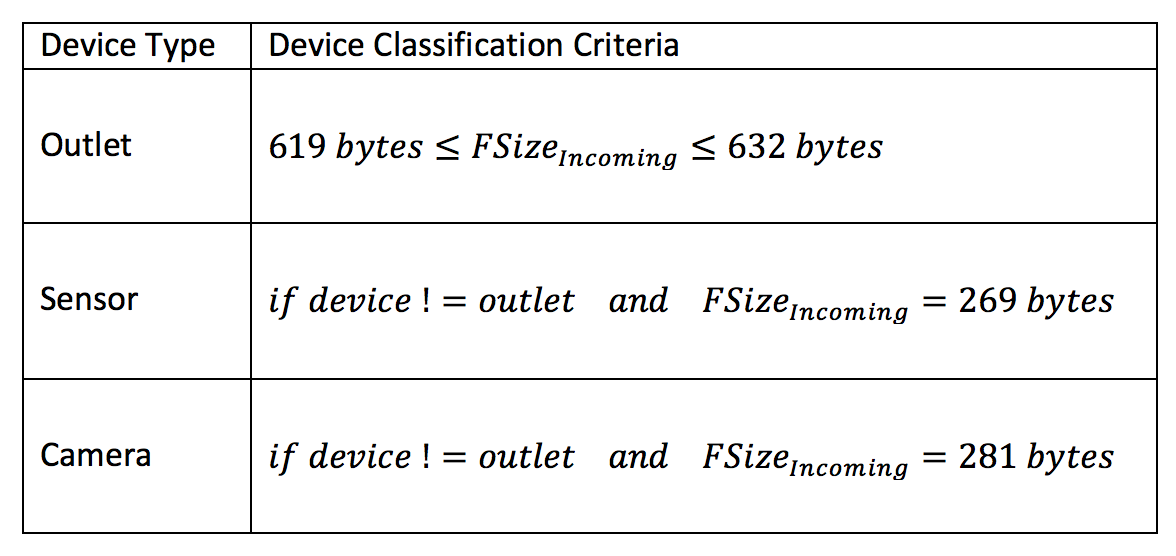
\includegraphics[height=2in]{deviceClassification}}
			\caption{Criteria used to classify devices}
			\label{fig:DeviceClassification}
		\end{center}
		\vspace{-0.2 in}
	\end{figure}
}

\newcommand{\figIdentificationToMini}{
	\begin{figure}[H]
		\begin{center}
			\makebox[\textwidth][c]{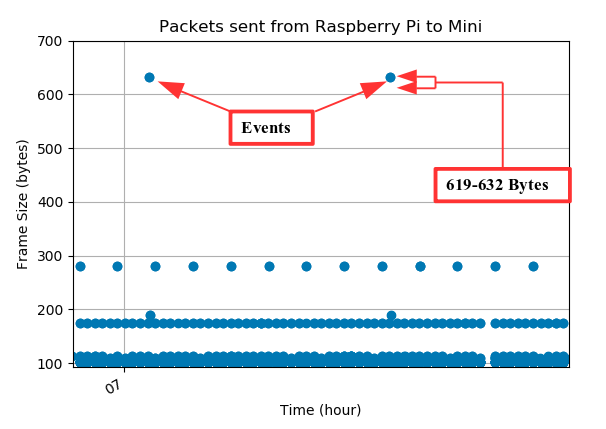
\includegraphics[width=5in]{identificationToMini}}
			\caption{Figure~\ref{fig:TrainingToDevice}(g) zoomed in on unique packet traffic used to identify outlet events}
			\label{fig:IdentificationToMini}
		\end{center}
		\vspace{-0.2 in}
	\end{figure}
}

\newcommand{\figIdentificationFromNetcam}{
	\begin{figure}[H]
		\begin{center}
			\makebox[\textwidth][c]{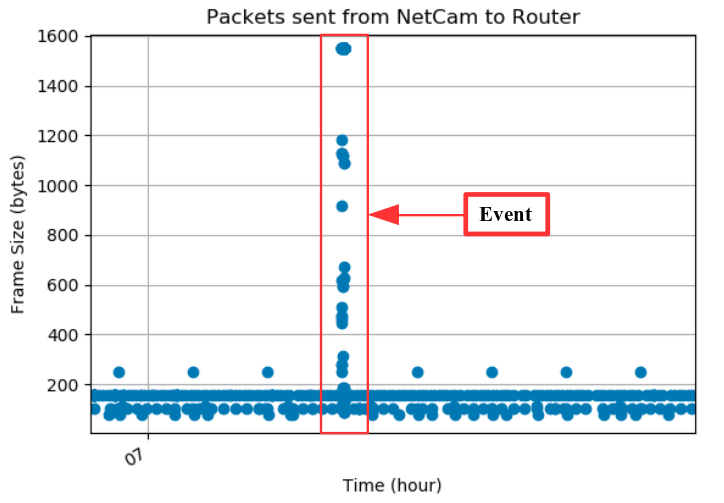
\includegraphics[width=5in]{identificationFromNetcam}}
			\caption{Figure~\ref{fig:TrainingFromDevice}(b) zoomed in on unique packet traffic used to identify camera events}
			\label{fig:IdentificationFromNetcam}
		\end{center}
		\vspace{-0.2 in}
	\end{figure}
}

\newcommand{\figIdentificationFromNetcamCum}{
	\begin{figure}[H]
		\begin{center}
			\makebox[\textwidth][c]{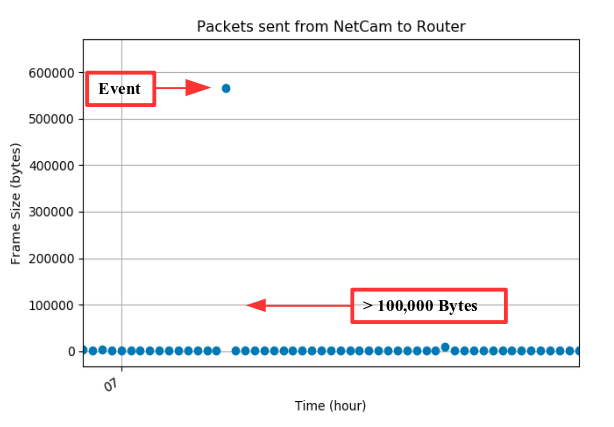
\includegraphics[width=5in]{identificationFromNetcamCum}}
			\caption{Figure~\ref{fig:TrainingFromDevice}(b) with one minute cumulative frame size zoomed in on unique packet traffic used to identify camera events}
			\label{fig:IdentificationFromNetcamCum}
		\end{center}
		\vspace{-0.2 in}
	\end{figure}
}

\newcommand{\figIdentificationFromMotion}{
	\begin{figure}[H]
		\begin{center}
			\makebox[\textwidth][c]{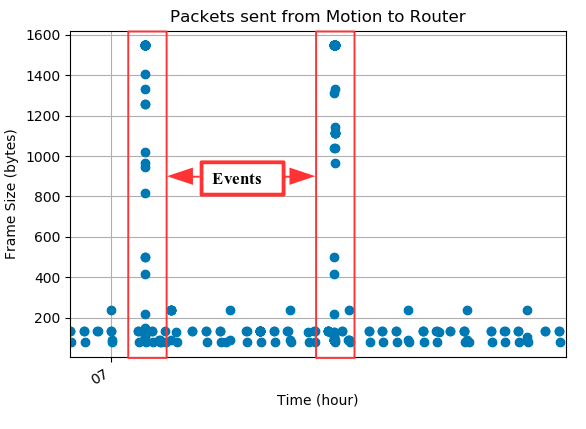
\includegraphics[width=5in]{identificationFromMotion}}
			\caption{Figure~\ref{fig:TrainingFromDevice}(a) zoomed in on unique packet traffic used to identify motion events}
			\label{fig:IdentificationFromMotion}
		\end{center}
		\vspace{-0.2 in}
	\end{figure}
}

\newcommand{\figIdentificationFromMotionCum}{
	\begin{figure}[H]
		\begin{center}
			\makebox[\textwidth][c]{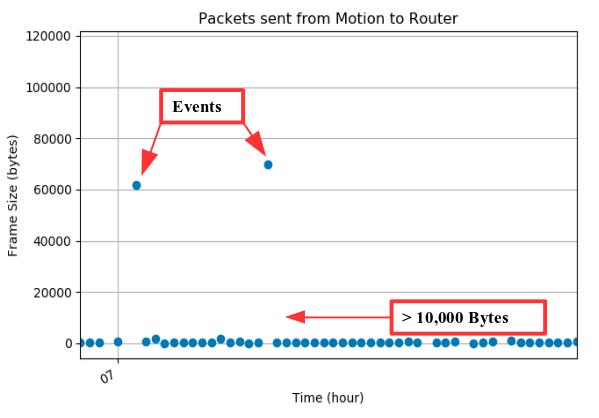
\includegraphics[width=5in]{identificationFromMotionCum}}
			\caption{Figure~\ref{fig:TrainingFromDevice}(a) with one minute cumulative frame size zoomed in on unique packet traffic used to identify motion events}
			\label{fig:IdentificationFromMotionCum}
		\end{center}
		\vspace{-0.2 in}
	\end{figure}
}

\newcommand{\figEventIdentification}{
	\begin{figure}[H]
		\begin{center}
			\makebox[\textwidth][c]{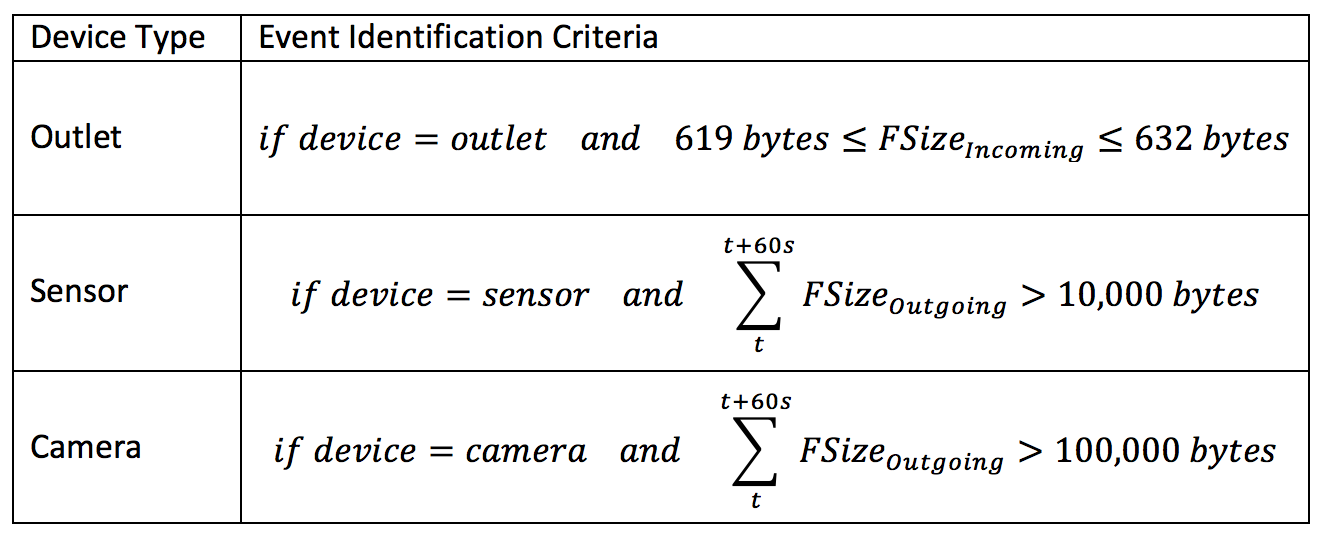
\includegraphics[height=2in]{eventIdentification}}
			\caption{Criteria used to identify events}
			\label{fig:EventIdentification}
		\end{center}
		\vspace{-0.2 in}
	\end{figure}
}

\newcommand{\figSubscribePacket}{
	\begin{figure}[H]
		\begin{center}
			\makebox[\textwidth][c]{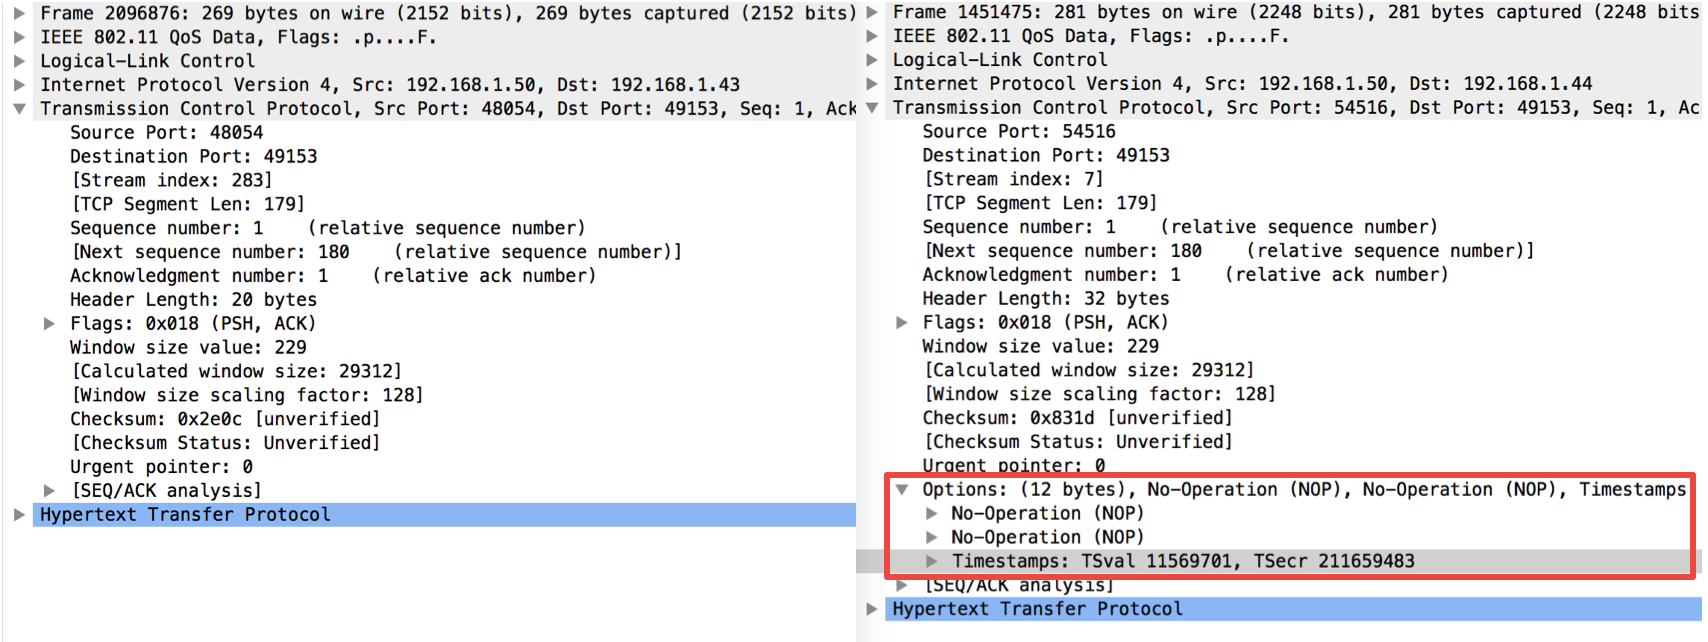
\includegraphics[width=\linewidth]{subscribePacket}}
			\caption{Decrypted \texttt{SUBSCRIBE} packets from Raspberry Pi to the NetCam and Motion devices depicting difference in frame length}
			\label{fig:SubscribePacket}
		\end{center}
		\vspace{-0.2 in}
	\end{figure}
}

\newcommand{\figPostPacket}{
	\begin{figure}[H]
		\begin{center}
			\makebox[\textwidth][c]{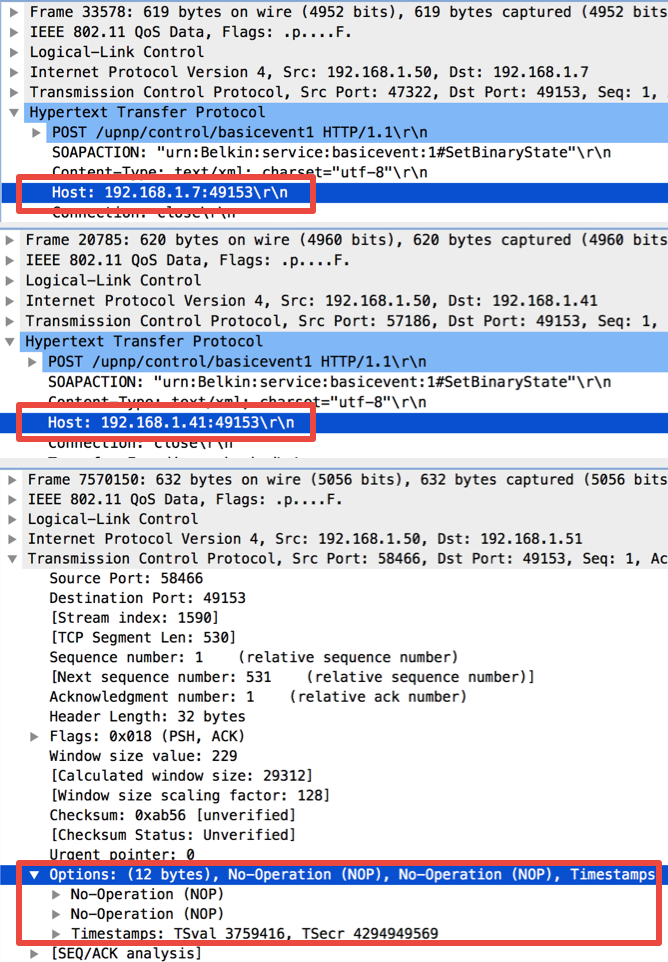
\includegraphics[width=.975\linewidth]{postPacket}}
			\caption{Decrypted \texttt{POST} packets from Raspberry Pi to the Switch4, Switch2, and Mini depicting differences in frame length}
			\label{fig:PostPacket}
		\end{center}
		\vspace{-0.2 in}
	\end{figure}
}

\newcommand{\figNetworkMap}{
	\begin{figure}[H]
		\begin{center}
			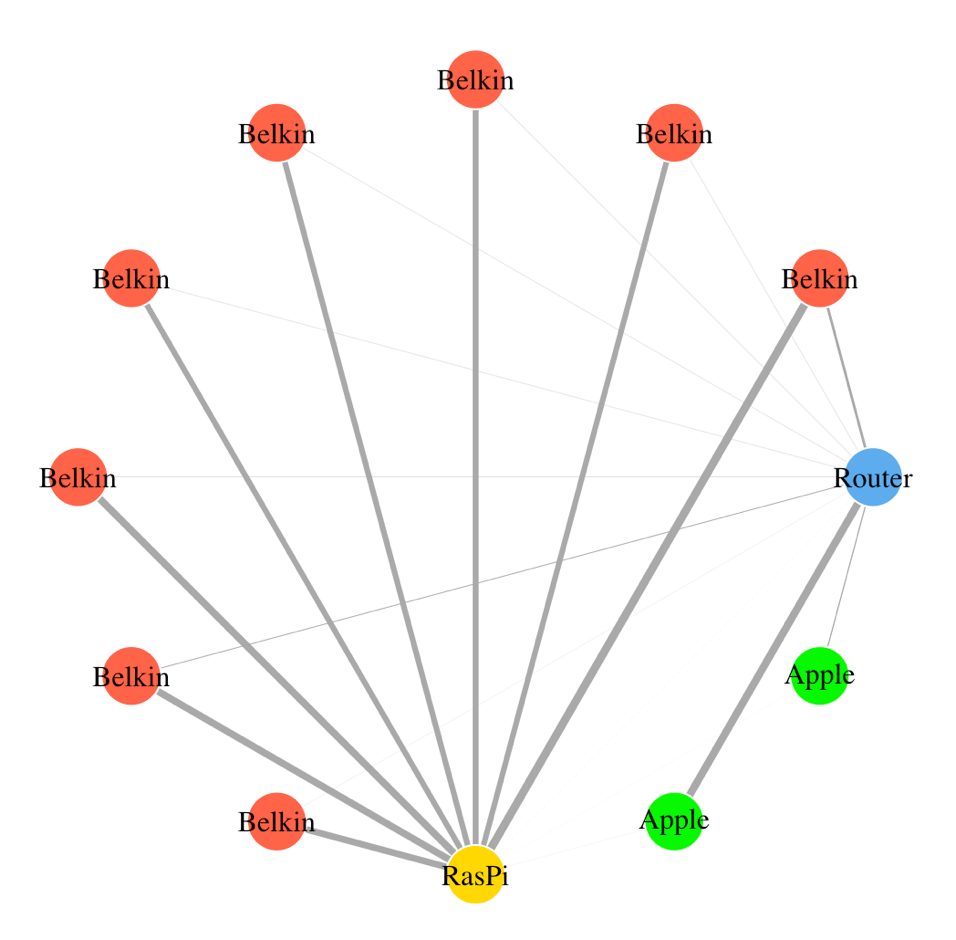
\includegraphics[width=5in]{networkMap}
			\caption{Network mapping of smart home architecture}
			\label{fig:NetworkMap}
		\end{center}
		\vspace{-0.2 in}
	\end{figure}
}

\newcommand{\figMiotlDiagram}{
	\begin{figure*}[h!]
		\begin{center}
			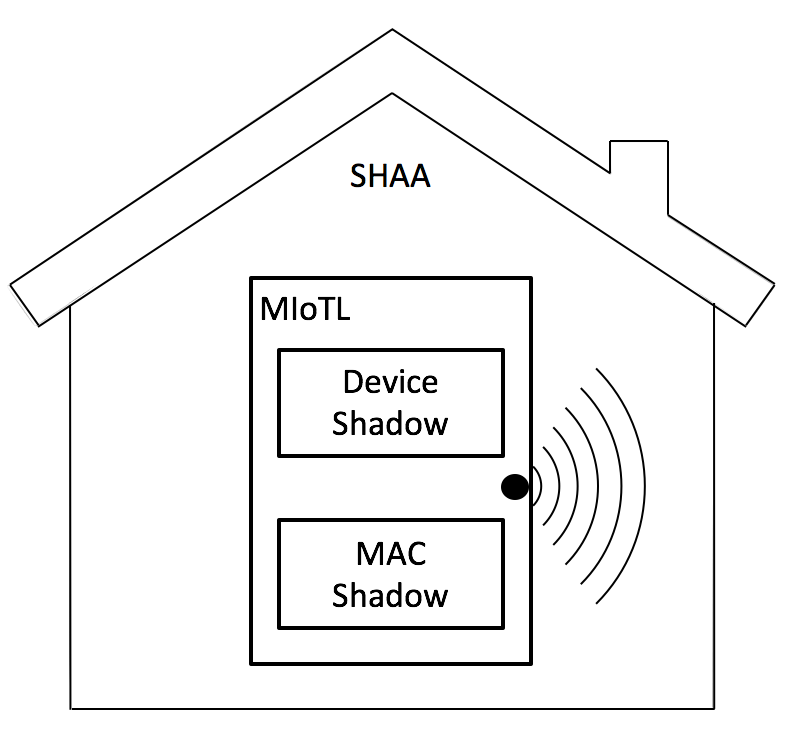
\includegraphics[width=3in]{miotlDiagram}
			\caption{Diagram of MIoTL tool components}
			\label{fig:MiotlDiagram}
		\end{center}
		\vspace{-0.2 in}
	\end{figure*}
}

\newcommand{\figSutCutDiagram}{
	\begin{figure*}[h!]
		\begin{center}
			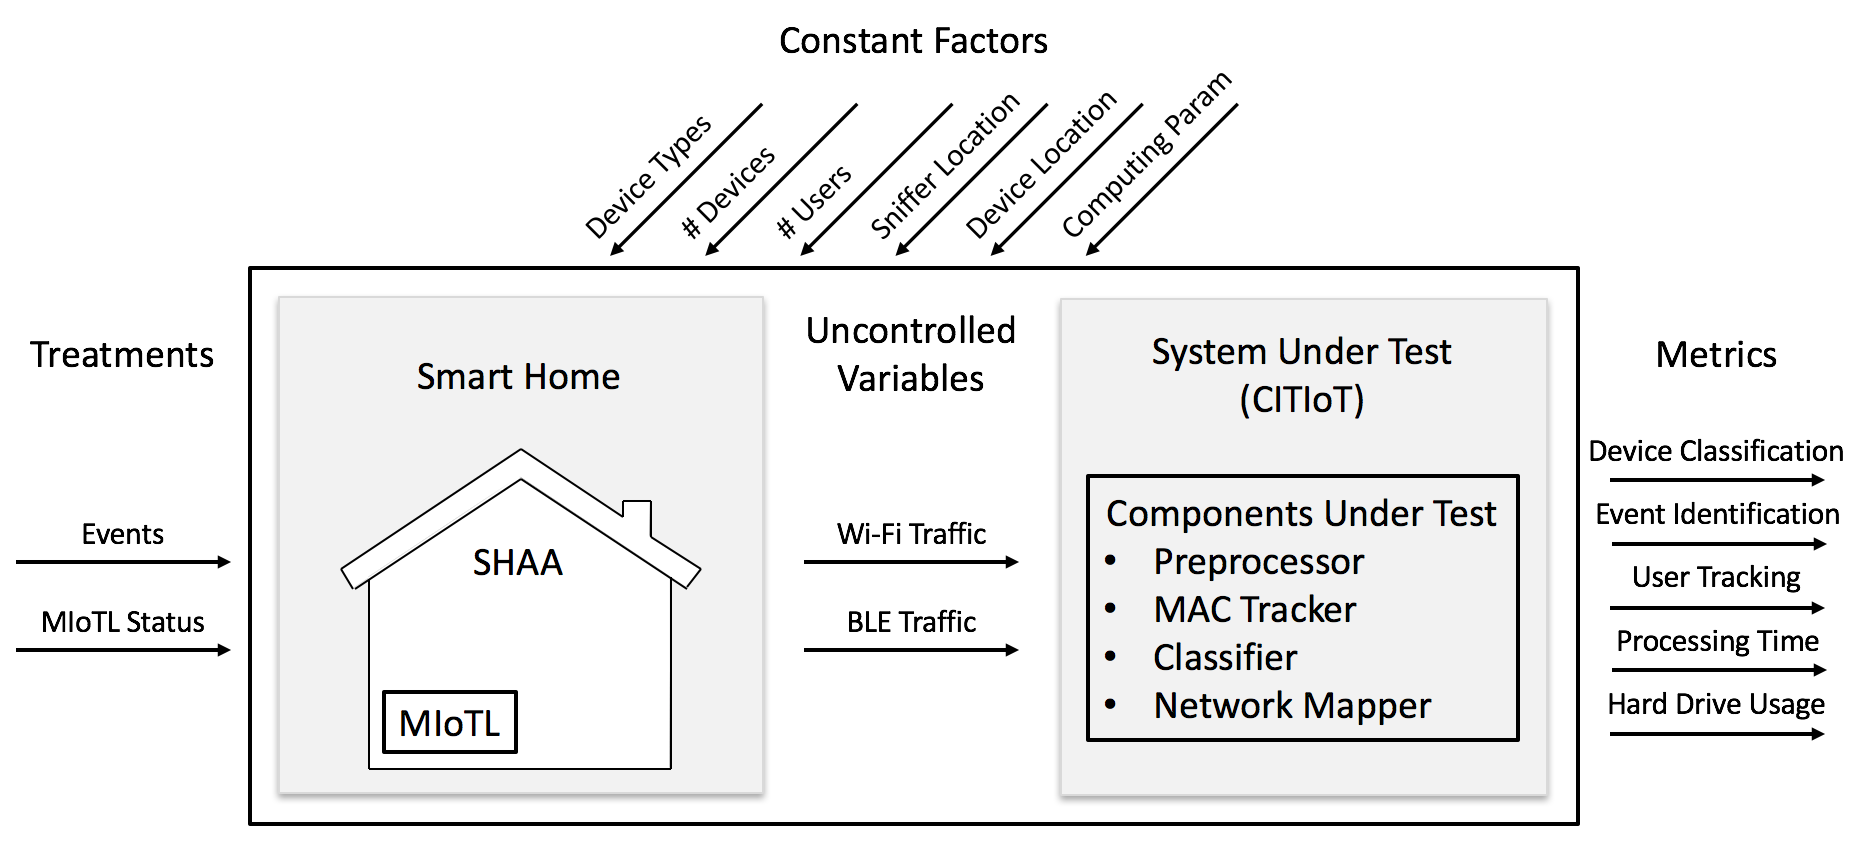
\includegraphics[width=\linewidth]{sutCutDiagram}
			\caption{System Under Test (SUT) and Component Under Test (CUT) diagram}
			\label{fig:SutCutDiagram}
		\end{center}
		\vspace{-0.2 in}
	\end{figure*}
}

\newcommand{\figShaaExperimentDiagram}{
	\begin{figure*}[h!]
		\begin{center}
			\includegraphics[width=\linewidth]{shaaExperimentDiagram}
			\caption{Approximate layout of devices within \ac{SHAA} for experimentation (not to scale)}
			\label{fig:ShaaExperimentDiagram}
		\end{center}
		\vspace{-0.2 in}
	\end{figure*}
}

\newcommand{\figSnifferExperimentSetup}{
	\begin{figure*}[h!]
		\begin{center}
			\includegraphics[width=\linewidth]{snifferExperimentSetup}
			\caption{Layout of sniffer antennae for experimentation}
			\label{fig:SnifferExperimentSetup}
		\end{center}
		\vspace{-0.2 in}
	\end{figure*}
}

\newcommand{\figDataCollectionFramework}{
	\begin{figure}[h!]
		\begin{center}
			\includegraphics[width=\linewidth, height = 5cm]{hostMachine}
			\caption{Data Collection Framework}
			\label{fig:DataCollectionFramework}
		\end{center}
		\vspace{-0.2 in}
	\end{figure}
}

\newcommand{\figSampleResults}{
\begin{figure}[H]
	\begin{center}
		\includegraphics[width=\linewidth]{sampleResults}
		\caption{Example graph comparing CITIoT events with actual events}
		\label{fig:SampleResults}
	\end{center}
	\vspace{-0.2 in}
\end{figure}
}

\newcommand{\figCitiot}{
	\begin{figure}[H]
		\begin{center}
			\makebox[\textwidth][c]{\includegraphics[width=5in]{citiot}}
			\caption{CITIoT Architecture}
			\label{fig:Citiot}
		\end{center}
		\vspace{-0.2 in}
	\end{figure}
}

\newcommand{\figReconScanning}{
	\begin{figure}[H]
		\begin{center}
			\makebox[\textwidth][c]{\includegraphics[width=5in]{reconScanning}}
			\caption{Scanning command along with output.}
			\label{fig:ReconScanning}
		\end{center}
		\vspace{-0.2 in}
	\end{figure}
}

\newcommand{\figNetworkMapping}{
	\begin{figure}[tbp]
		\begin{center}
			\includegraphics[width=3in, height=7cm]{networkMapping}
			\caption{Network mapping of smart home architecture; thicker lines mean stronger correlation between devices.}
			\label{fig:NetworkMapping}
		\end{center}
		\vspace{-0.2 in}
	\end{figure}
}

\newcommand{\figMethodologyOverview}{
	\begin{figure}[H]
		\begin{center}
			\makebox[\textwidth][c]{\includegraphics[width=6in]{methodologyOverview}}
			\caption{Overall scenario setup.}
			\label{fig:MethodologyOverview}
		\end{center}
		\vspace{-0.2 in}
	\end{figure}
}

\newcommand{\figDeviceId}{
	\begin{figure}[H]
	\centering
		\begin{minipage}{.5\textwidth}
			\centering
			\includegraphics[width=1\linewidth]{deviceIdOutlet}
			\caption{Outlet device.}
			\label{fig:DeviceIdOutlet}
		\end{minipage}%
		\begin{minipage}{.5\textwidth}
			\centering
			\includegraphics[width=1\linewidth]{deviceIdSensor}
			\caption{Sensor device.}
			\label{fig:DeviceIdSensor}
		\end{minipage}
		\begin{minipage}{.5\textwidth}
			\centering
			\includegraphics[width=1\linewidth]{deviceIdCamera}
			\caption{Camera device.}
			\label{fig:DeviceIdCamera}
		\end{minipage}
	\end{figure}
}


\newcommand{\figExamplePlotOne}{
	\begin{figure}[H]
		\begin{center}
			\makebox[\textwidth][c]{\includegraphics[width=4.5in]{examplePlot1}}
			\caption{Example Plot One: Event Identification}
			\label{fig:ExamplePlotOne}
		\end{center}
		\vspace{-0.2 in}
	\end{figure}
}

\newcommand{\figExamplePlotTwo}{
	\begin{figure}[H]
		\begin{center}
			\makebox[\textwidth][c]{\includegraphics[width=4.5in]{examplePlot2}}
			\caption{Example Plot Two: Time User is Home}
			\label{fig:ExamplePlotTwo}
		\end{center}
		\vspace{-0.2 in}
		\end{figure}
}

\newcommand{\figafitStyle}{\begin{figure}[tbp]
 \begin{center}
    \includegraphics[width=6in]{myFirstLaTeXafit}
     \caption{Recompile using afitThesis.sty, the AFIT
     thesis style file.}
     \label{fig:afitStyle}
 \end{center}
\end{figure}
}


\newcommand{\figtitlePage}{\begin{figure}[tbp]
 \begin{center}
    \includegraphics[width=6in]{titlePage}
     \caption{Enter student data in titlePage.tex to customize the
     document's first pages.}
     \label{fig:titlePage}
 \end{center}
\end{figure}
}

\newcommand{\figmyFlypage}{\begin{figure}[tbp]
 \begin{center}
    \includegraphics[width=6in]{myFlypage}
     \caption{Here we have compiled the first four page of a thesis.}
     \label{fig:myFlypage}
 \end{center}
\end{figure}
}

\newcommand{\figmyFirstAbstract}{\begin{figure}[tbp]
 \begin{center}
    \includegraphics[width=6in]{myFirstAbstract}
     \caption{Add an abstract to the front matter of your thesis.}
     \label{fig:myFirstAbstract}
 \end{center}
\end{figure}
}

\newcommand{\figmyFigures}{\begin{figure}[tbp]
 \begin{center}
    \includegraphics[width=5in]{myFigures}
     \caption{Consider defining all your figures in one file.}
     \label{fig:myFigures}
 \end{center}
\end{figure}
}


\newcommand{\figmyFirstFigures}{\begin{figure}[tbp]
 \begin{center}
    \includegraphics[width=6in]{myFirstFigures}
     \caption{Add figures in the main matter of your document; fill in
     the document around your graphics.}
     \label{fig:myFirstFigures}
 \end{center}
\end{figure}
}

\newcommand{\figmyFirstBibTeX}{\begin{figure}[tbp]
 \begin{center}
    \includegraphics[width=6in]{myFirstBibTeX}
     \caption{Add your bibliography.}
     \label{fig:myFirstBibTeX}
 \end{center}
\end{figure}
}




\newcommand{\tableWifiDevices}{
\begin{table}[H]
	\centering
	\caption{Wi-Fi Devices.}\label{tbl:WifiDevices}
	\makebox[\textwidth][c]{\begin{tabular} {| c | c | c | c | c | c |}
		\hline
		\thead{ID} & \thead{Manuf} & \thead{Device Type} & \thead{Device Name} &  \thead{MAC} & \thead{IP Address} \\ 
		\hline
		w$_1 $ & Calix & Wireless Router & Moria & EC:4F:82:73:D1:1A & - \\
		\hline
		w$_2 $ & Belkin & Camera & NetCam & EC:1A:59:E4:FD:41 & 192.168.1.44 \\
		\hline
		w$_3 $ & Belkin & Outlet & Switch1 & B4:75:0E:0D:33:D5 & 192.168.1.40 \\
		\hline
		w$_4 $ & Belkin & Outlet & Switch2 & B4:75:0E:0D:94:65 & 192.168.1.41 \\
		\hline
		w$_5 $ & Belkin & Outlet & Switch3 & 94:10:3E:2B:7A:55 & 192.168.1.42 \\
		\hline
		w$_6 $ & Belkin & Outlet & Switch4 & 14:91:82:C8:6A:09 & 192.168.1.7 \\
		\hline
		w$_7 $ & Belkin & Motion Sensor & Motion & EC:1A:59:F1:FB:21 & 192.168.1.43 \\
		\hline
		w$_8 $ & Belkin & Outlet & Insight & 14:91:82:24:DD:35 & 192.168.1.47 \\
		\hline
		w$_9 $ & WeMo & Outlet & Mini & 60:38:E0:EE:7C:E5 & 192.168.1.51 \\
		\hline
		w$_{10} $ & Raspberry Pi 3B & Computer & Pi & B8:27:EB:09:1A:81 & 12.168.1.50 \\
		\hline
		w$_{11} $ & Apple & iPhone 6+ & Steves-phone & A0:18:28:33:34:F8 & 192.168.1.4 \\
		\hline
		w$_{12} $ & Apple & TV 2 & Apple-TV & 08:66:98:ED:1E:19 & 192.168.1.54 \\
		\hline
	\end{tabular}}
\end{table}
}

\newcommand{\tableWifiDeviceShort}{
	\begin{table}[tbp]
		\centering
		\caption{Wi-Fi Devices.}\label{tbl:WifiDevicesShort}
			\begin{tabular} {| c | c | c | c |}
				\hline
				\thead{ID} & \thead{Manuf} & \thead{Device Type} & \thead{Device Name} \\ 
				\hline
				w$_1 $ & Calix & Wireless Router & Prancing Pony  \\
				\hline
				w$_{2-5} $ & Belkin & Outlet & Switch1-4 \\
				\hline
				w$_6 $ & WeMo & Outlet & Mini  \\
				\hline
				w$_7 $ & Belkin & Outlet & Insight  \\
				\hline
				w$_8 $ & Belkin & Motion Sensor & Motion \\
				\hline
				w$_9 $ & Belkin & Camera & NetCam  \\
				\hline
				w$_{10} $ & Raspberry Pi 3B & Computer & Pi \\
				\hline
				w$_{11} $ & Apple & iPhone 6+ & Steves-phone  \\
				\hline
				w$_{12} $ & Apple & TV 2 & Apple-TV \\
				\hline
			\end{tabular}
	\end{table}
}

\newcommand{\tableBtleDevicesShort}{
	\begin{table}[tbp]
		\centering
		\caption{BLE Devices.}\label{tbl:BtleDevicesShort}
\begin{tabular}{|c|c|c|c|}
	\hline
	\thead{ID} & \thead{Manuf} & \thead{Device Type} & \thead{Device Name} \\
	\hline
	b$ _1 $ & Elgato & Indoor Temperature & Eve Room \\
	\hline
	b$ _2 $ & Elgato & Outdoor Temperature & Eve Weather \\
	\hline
	b$ _3 $ & Elgato & Motion Sensor & Eve Motion \\
	\hline
	b$ _4 $ & Elgato & Outlet & Eve Energy \\
	\hline
	b$ _5 $ & Elgato & Door Sensor & Eve Door \\
	\hline
	b$ _6 $ & Instant Pot & Smart Cooker & Instant Pot \\
	\hline
	b$ _7 $ & MPow & Lightbulb & Playbulb \\
	\hline
	b$ _8 $ & ZKTeco & Lock & BioLock \\
	\hline
	b$ _{9} $ & BitLock & Lock & Bike lock \\
	\hline
	b$ _{10} $ & SafeTech & Gunsafe & Gunsafe \\
	\hline
	b$ _{11} $ & Apple & iPhone 6+ & Steves-phone \\
	\hline
	b$ _{12} $ & Apple & TV 2 & Apple TV \\
	\hline
\end{tabular}
\end{table}
}

\newcommand{\tableDeviceClassifier}{
	\begin{table*}[tbp]
		\centering
		\caption{Classifier Criterion.}\label{tbl:DeviceClassifier}
		\begin{tabular} {| c | c | c |}
			\hline
			\thead{Device Type} & \thead{Device Classification} & \begin{tabular}{@{}c@{}}\thead{Event Identification} \\ (Relies on Device Classification)\end{tabular} \\
			\hline
			Outlet & $FSize_{in} > 650\ bytes$ & $1,000 > FSize_{in} > 600\ bytes$ \\
			\hline
			Sensor & $device\ != outlet\ and\ all\ FSize_{in} < 275\ bytes$ & $100,000>\sum\limits_{t}^{t+1}FSize_{out}>10,000\ bytes$\\
			\hline
			Camera & $device\ != outlet\ and\ 275 < FSize_{in} < 300\ bytes$ & $\sum\limits_{t}^{t+1}FSize_{out}>100,000\ bytes$\\
			\hline
		\end{tabular}
	\end{table*}
}

\newcommand{\tableBtleDevices}{
\begin{table}[H]
	\centering
	\caption{BLE Devices.}\label{tbl:BtleDevices}
	\makebox[\textwidth][c]{\begin{tabular}{| c | c|c|c|}
		\hline
		\thead{ID} & \thead{Manuf} & \thead{Device Type} & \thead{Device Name} \\
		\hline
		b$ _1 $ & Elgato & Indoor Temperature & Eve Room \\
		\hline
		b$ _2 $ & Elgato & Outdoor Temperature & Eve Weather \\
		\hline
		b$ _3 $ & Elgato & Motion Sensor & Eve Motion \\
		\hline
		b$ _4 $ & Elgato & Outlet & Eve Energy \\
		\hline
		b$ _5 $ & Elgato & Switch & Eve Light \\
		\hline
		b$ _6 $ & Elgato & Door Sensor & Eve Door \\
		\hline
		b$ _7 $ & Instant Pot & Smartcooker & Instant Pot \\
		\hline
		b$ _8 $ & MPow & Lightbulb & Playbulb \\
		\hline
		b$ _9 $ & ZKTeco & Lock & BioLock \\
		\hline
		b$ _{10} $ & BitLock & Lock & Bike lock \\
		\hline
		b$ _{11} $ & SafeTech & Gunsafe & Gunsafe \\
		\hline
		b$ _{12} $ & Apple & iPhone 6+ & Steves-phone \\
		\hline
		b$ _{13} $ & Apple & TV 2 & Apple TV \\
		\hline
	\end{tabular}}
\end{table}
}

\newcommand{\tablePerformanceMetrics}{
	\begin{table}[H]
		\centering
		\caption{Performance Metrics}
		\makebox[\textwidth][c]{\begin{tabular}{|c|c|c|c|}
			\hline
			\thead{Metric} & \thead{Units} & \thead{Accepted Range} & \thead{Expected Value} \\
			\hline
			DCSR (Device Classification Success Rate) & \% & 0 to 100 & $>$ 75\% \\
			\hline
			EISR (Event Identification Success Rate) & \% & 0 to 100 & $>$ 75\% \\
			\hline
			EIFP (Event Identification False Positives) & \% & 0 to 100 & $>$ 75\% \\
			\hline
			EIFN (Event Identification False Negatives) & \% & 0 to 100 & $>$ 75\% \\
			\hline
			ULSR (User Location Success Rate) & \% & 0 to 100 & $>$ 75\% \\
			\hline
			CT (Completion Time) & minutes & 0 to $\infty$ & $<$ 120 minutes \\
			\hline
			HDU (Hard Drive Usage) & bytes & 0 to $\infty$ & $<$ 20 GB \\
			\hline
		\end{tabular}}
		\label{tbl:PerformanceMetrics}
	\end{table}
}

\newcommand{\tableEvents}{
	\begin{table}[h!]
		\centering
		\caption{Experiment Events}\label{tbl:Events}
		\begin{tabular}{|c|c|c|c|}
			\hline
			\ & \thead{Device Name} & \thead{Action} & \thead{Protocol} \\
			\hline
			1 & Bike Lock & Unlock & BLE \\
			\hline
			2 & BioLock & Unlock & BLE \\
			\hline
			3 & Instant Pot & Turn on & BLE \\
			\hline
			4 & Instant Pot & Turn off & BLE \\
			\hline
			5 & Gunsafe  & Open & BLE \\
			\hline
			6 & Gunsafe  & Close & BLE \\
			\hline
			7 & Eve Room & Get temperature in living room & BLE \\
			\hline
			8 & Eve Weather & Get temperature on patio & BLE \\
			\hline
			9 & Eve Door & Open & BLE \\
			\hline
			10 & Eve Door & Close & BLE \\
			\hline
			11 & Eve Energy & Turn on & BLE \\
			\hline
			12 & Eve Energy & Turn off & BLE \\
			\hline
			13 & Eve Motion & Activate motion sensor & BLE \\
			\hline
			14 & Playbulb & Turn on & BLE \\
			\hline
			15 & Playbulb & Turn off & BLE \\
			\hline
			16 & Switch1 & Turn on & Wi-Fi \\
			\hline
			17 & Switch1 & Turn off & Wi-Fi \\
			\hline
			18 & Switch2 & Turn on & Wi-Fi \\
			\hline
			19 & Switch2 & Turn off & Wi-Fi \\
			\hline
			20 & Switch3 & Turn on & Wi-Fi \\
			\hline
			21 & Switch3 & Turn off & Wi-Fi \\
			\hline
			22 & Switch4 & Turn on & Wi-Fi \\
			\hline
			23 & Switch4 & Turn off & Wi-Fi \\
			\hline
			24 & Mini & Turn on & Wi-Fi \\
			\hline
			25 & Mini & Turn off & Wi-Fi \\
			\hline
			26 & Insight & Turn on & Wi-Fi \\
			\hline
			27 & Insight & Turn off & Wi-Fi \\
			\hline
			28 & NetCam & Activate motion & Wi-Fi \\
			\hline
			29 & Motion & Activate motion sensor & Wi-Fi \\
			\hline
			30 & Steves-phone & Leave house & Wi-Fi and BLE \\
			\hline
			31 & Steves-phone & Arrive House & Wi-Fi and BLE \\
			\hline
		\end{tabular}
	\end{table}
}

\newcommand{\tableTreatments}{
	\begin{table}[h!]
		\centering
		\caption{Experiment Treatments}
		\begin{tabular}{|c|c|c|}
			\hline
			\thead{Trial} \# & \thead{Events Administered} & \thead{MIoTL Status} \\
			\hline
			1-5 & 1-31 & Off \\
			\hline
			6 & 16-31 & On \\
			\hline
		\end{tabular}
		\label{tbl:Treatments}
	\end{table}
}

\newcommand{\tableTools}{
\begin{table}[H]
	\centering
	\caption{Wi-Fi and \ac{BLE} tools used throughout this work.}
	\label{tbl:Tools}
	\makebox[\textwidth][c]{\begin{tabular}{|c|c|p{8cm}|}
		\hline
		\textbf{Tool Name} & \textbf{Version}     & \textbf{Description} \\ 
		\hline
		Ubertooth One      & Firmware: 2017-03R2  & Bluetooth sniffer with open-source firmware and hardware \cite{Ubertooth} \\
		\hline
		BlueZ              & 5.43                 & Linux Bluetooth stack with utilities to scan for \ac{BLE} devices and transmit packets \cite{Bluez}\\
		\hline
		Plugable USB	   & 2.0				  & Commercial Broadcom BCM20702-based Bluetooth adapter to communicate with Bluetooth Devices \\
		\hline
		Alfa Card		   & AWUS036ACH			  & 802.11ac Wireless Adapter\\
		\hline
		Airodump-ng		   & Aircrack-ng 1.2	  & Wi-Fi network security tool to capture raw 802.11 frames\\
		\hline
		Python			   & 2.7.10				  & Programming language used in scripting\\
		\hline
		Pyshark			   & 0.3.7.8			  & Python wrapper allowing python packet parsing with wireshark dissectors \cite{pyshark}\\
		\hline
		Scapy			   & 2.3.3				  & Interactive packet manipulation tool used to send or receive 802.11 packets \cite{scapy}\\
		\hline
	\end{tabular}}
\end{table}
}

\newcommand{\tableBleResults}{
	\begin{table}[tbp]
		\centering
		\caption{Summary of \ac{BLE} Results.}
		\label{tbl:BleResults}
		\begin{tabular}{|c|c|c|c|c|}
			\hline
			\textbf{Date} & \textbf{True Pos} & \textbf{False Neg} & \textbf{False Pos} & \textbf{\# Events} \\ 
			\hline
			Day 1 & No Data & No Data & No Data & No Data \\
			\hline
			Day 2 & 37 & 5 & 5 & 42\\
			\hline
			Day 3 & 40 & 1 & 3 & 41\\
			\hline
			Day 4 & 36 & 0 & 9 & 36\\
			\hline
			Day 5 & 31 & 2 & 4 & 33\\
			\hline
			\hline
			Average & 36 & 2 & 5.25 & 38\\
			\hline
		\end{tabular}
	\end{table}
}

\newcommand{\tableWifiResults}{
	\begin{table}[tbp]
		\centering
		\caption{Summary of Wi-Fi Results.}
		\label{tbl:WifiResults}
		\begin{tabular}{|c|c|c|c|c|}
			\hline
			\textbf{Date} & \textbf{True Pos} & \textbf{False Neg} & \textbf{False Pos} & \textbf{\# Events} \\ 
			\hline
			Day 1 & 31 & 0 & 0 & 31 \\
			\hline
			Day 2 & 34 & 1 & 1 & 35 \\
			\hline
			Day 3 & 34 & 3 & 1 & 37 \\
			\hline
			Day 4 & 35 & 2 & 1 & 37 \\
			\hline
			Day 5 & 28 & 4 & 1 & 33 \\
			\hline
			\hline
			Average & 32.4 & 2 & 1 & 34.6\\
			\hline
		\end{tabular}
	\end{table}
}

\newcommand{\tableDeviceID}{
\begin{table}[H]
	\centering
	\caption{Device Classification Criterion.}
	\label{tab:DeviceID}
	\makebox[\textwidth][c]{\includegraphics[width=5in]{deviceID}}
\end{table}
}

\newcommand{\tableEventID}{
	\begin{table}[H]
		\centering
		\caption{Event Identification Criterion.}
		\label{tab:EventID}
		\makebox[\textwidth][c]{\includegraphics[width=5in]{eventID}}
	\end{table}
}


\newcommand{\tabRadiometricQuantities}{
\begin{table}[htbp]
  \centering
  \caption{Radiometric Quantities in SI units.}\label{tab:RadiometricQuantities}
\begin{tabular}{|c|c|c|c|}
  \hline
  Symbol & Name & Units & Definition \\
  \hline
  $A$ & area & cm$^2$ & projected area of source \\
  $R$ & length & cm & distance between source and \\
  &  &  & collection optic \\
  $\theta$ & linear angle & rad & angle between source and  \\
  &  &  & collection optic \\
  $\Omega$ & solid angle & sr & $d\Omega = \frac{dA}{R^2}$ \\
  $\phi$ & flux & W & radiant energy reaching collection optic \\
   &  &  & per unit time \\
  $L$ & radiance & $\frac{W}{cm^2 sr}$ & $L = \frac{\partial^2 \phi}{\partial A \cos \theta \partial \Omega}$ \\
  $I$ & intensity & $\frac{W}{sr}$ & $I = \frac{\partial \phi}{\partial \Omega} = \int_A L \cos \theta dA$ \\
  $F$ & irradiance & $\frac{W}{cm^2}$ & $F = \frac{\partial \phi}{\partial A_d}$ $A_d = $ area of collection optic \\
  $B_{\bar{\nu}}$ & Planck distribution & $\frac{W}{cm^2 sr cm^{-1}}$ & $B_{\bar{\nu}} d\bar{\nu} = \frac{2 h c^2 {\bar{\nu}}^3}{\exp(\frac{h c \bar{\nu}}{k_B T}) - 1} d\bar{\nu}$ \\
  \hline
\end{tabular}
\end{table}
}


\newcommand{\tabFullSpectrumInitialFit}{
\begin{table}
\caption{Initial analysis with full spectrum fit of r, T, H$_2$0,
CO$_2$, CO fit parameters} \label{tbl:FullSpectrumInitialFit}
\begin{center}
\begin{tabular}{|c|c|c|c|c|c|}\hline
Data Set &  ENGINE02 &  ENGINE03 &  SS01 &  SS02 &  SS03 \\ \hline
r (cm) &    13500 & 40.9 &  122 &   140 &   159 \\ \hline
T (K) & 437 &   881 &   1320 &  1220 &  1200 \\ \hline
H$_2$0 &   1.68E+19 &  3.31E+21 &  1.45E+18 &  1.73E+18 &  1.77E+18 \\ \hline
CO$_2$ &   4.5E+19 &   4.17E+15 &  2.06E+18 &  2.11E+18 &  1.78E+18 \\ \hline
CO &    3.4E+17 &   6.85E+13 &    2.35E+17 &  2.91E+17 &  3.65E+17 \\ \hline
H$_2$O:CO$_2$ &   3.73E+2 & 7.94E+5 &  7.04E-1 & 8.20E-1 & 9.94E-1 \\ \hline
H$_2$O:CO &    4.94E+1 &  4.83E+7 &  6.17 &  5.95 &  4.85 \\ \hline
CO$_2$:CO &    1.32E+2 &  6.09E+1 &  8.77 &  7.25 &  4.88 \\ \hline
H:C &   7.41E-1 & 1.56E+6 &  1.26 &   1.44 &  1.65 \\ \hline
\end{tabular}
\end{center}
\end{table}
}

\newcommand{\tabFullSpectrumSteadyStateFit}{
\begin{table}
\caption{Subsequent analysis with r = 150 cm, and full spectrum
fit of T, H$_2$0, CO$_2$, CO fit parameters}
\label{tbl:FullSpectrumSteadyStateFit}
\begin{center}
\begin{tabular}{|c|c|c|c|}\hline
Data Set &  SS01 &  SS02 &  SS03 \\ \hline
r (cm) &    150 &   150 &   150 \\ \hline
T (K) & 1390 &  1180 &  1210 \\ \hline
H20 &   9.43E+17 &  1.98E+18 &  1.77E+18 \\ \hline
CO$_2$ &   1.18E+18 &  2.38E+18 &  1.88E+18 \\ \hline
CO &    1.58E+17 &  3.09E+17 &  3.68E+17 \\ \hline
H$_2$O:CO$_2$ &   7.99E-1 &   8.32E-1 &   9.41E-1 \\ \hline
H$_2$O:CO &    5.97 &  6.41 &  4.81 \\ \hline
CO$_2$:CO &    7.47 &  7.70 &  5.11 \\ \hline
H:C &   1.41 &  1.47 &  1.57 \\ \hline
\end{tabular}
\end{center}
\end{table}
}

\newcommand{\tabFullSpectrumSteadyStateFitConstantRT}{
\begin{table}
\caption{Subsequent analysis with r, T fixed (r = 150 cm, T = 1150
K), and full spectrum fit of H$_2$0, CO$_2$, CO fit parameters}
\label{tbl:FullSpectrumSteadyStateFitConstantRT}
\begin{center}
\begin{tabular}{|c|c|c|c|}\hline
Data Set &  SS01 &  SS02 &  SS03 \\ \hline
r (cm) &    150 &   150 &   150 \\ \hline
T (K) & 1150 &  1150 &  1150 \\ \hline
H20 &   2.24E+18 &  2.22E+18 &  2.36E+18 \\ \hline
CO$_2$ &   3.39E+18 &  2.8E+18 &   2.55E+18 \\ \hline
CO &    3.61E+17 &  3.58E+17 &  4.53E+17 \\ \hline
H$_2$O:CO$_2$ &   6.61E-1 &   7.93E-1 &   9.25E-1 \\ \hline
H$_2$O:CO &    6.20 &  6.20 &  5.21 \\ \hline
CO$_2$:CO &    9.39 &  7.82 &  5.63 \\ \hline
H:C &   1.19 &  1.41 &  1.57 \\ \hline
\end{tabular}
\end{center}
\end{table}
}

\usepackage[outdir=./]{epstopdf}

\begin{document}
	\begin{acronym}
		\acro {BLE} {Bluetooth Low Energy}
		\acro {SIG} {Special Interest Group}
		\acro {BR/EDR} {Basic Rate/Enhanced Data Rate}
		\acro {IoT} {internet of things}
		\acro {CI} {critical infrastructure}
		\acro {WSN} {Wireless Sensor Network}
		\acro {ATT} {Attribute Protocol}
		\acro {GATT} {Generic Attribute Profile}
		\acro {SM} {Security Manager}
		\acro {LTK} {Long Term Key}
		\acro {CSRK} {Connection Signature Resolving Key}
		\acro {IRK} {Identity Resolving Key}
		\acro {AES} {Advanced Encryption Standard}
		\acro {TK} {Temporary Key}
		\acro {STK} {Short-Term Key}
		\acro {ECDH} {Elliptic Curve Diffie Hellman}
		\acro {CE} {Connection Events}
		\acro {CRC} {Cyclic Redundancy Check}
		\acro {SCA} {sleep clock accuracy}
		\acro {RSSI} {Received Signal Strength Indicator}
		\acro {MAC} {Media Access Control}
		\acro {CRM} {Customer Relationship Management}
		\acro {SSID} {Service Set Identifiers}
		\acro {AP} {access point}
		\acro {CITIoT} {Classification, Identification, and Tracking of \ac{IoT}}
		\acro {MIoTL} {Mitigation of \ac{IoT} Leakage}
		\acro {SHAA} {Smart Home Automation Architecture}
		\acro {SUT} {System Under Test}
		\acro {CUT} {Component Under Test}
		\acro {DCSR} {Device Classification Success Rate}
		\acro{EISR} {Event Identification Success Rate}
		\acro{EIFP} {Event Identification False Positives}
		\acro{EIFN} {Event Identification False Negatives}
		\acro{ULSR} {User Location Success Rate}
		\acro{PT} {Processing Time}
		\acro{HDU} {Hard Drive Usage}
		\acro{COTS} {commercial off-the-shelf}
	\end{acronym}
\mainmatter
	\chapter{Methodology}
		\section{Problem/Objective}
		This research aims to demonstrate how data leakage in smart home environments enable an eavesdropper to classify \ac{IoT} devices, track user's movements, map networks, and identify events within the smart home. It also seeks to show how a smart home user can defend against these attacks. These goals are enabled through the implementation of the \ac{CITIoT} and \ac{MIoTL} tools respectively. The experiment presented in this section functions as an evaluation of these tools in a realistic smart home environment, testing how accurately the \ac{CITIoT} tool operates against the \ac{SHAA} and how well \ac{MIoTL} mitigates these attacks. Specifically, the experimentation attempts to accomplish four objectives:
		\begin{enumerate}
			\item Determine the ability of an observer to accurately classify smart home devices.*
			\item Examine with what success rate events can be identified.*
			\item Measure the capability to track when users are in the smart home.*
			\item Evaluate processing time and storage requirements.
			
			\begin{footnotesize}
			* Objective is fulfilled in two states: when the \ac{MIoTL} tool is activated and when it is not.
			\end{footnotesize}
		\end{enumerate}
		The evaluation results will provide consumers with an understanding of data leakage in smart home environments and a method to defend against these vulnerabilities.
		
		\section{System Under Test}
		Figure~\ref{fig:SutCutDiagram} displays the \ac{SUT} and \ac{CUT} diagram. Section \ref{treatments} describes the experiment treatments which include a user performing actions from a script to interact with the smart home environment and the operation of the \ac{MIoTL} tool. Section~\ref{constantFactors} discusses the constant factors that do not change throughout the experiment such as computing parameters and the number of devices. The actual Wi-Fi and \ac{BLE} traffic collected by the \ac{CITIoT} tool is considered uncontrolled and is examined in Section~\ref{uncontrolledVariables}. The components tested include the preprocessor, \ac{MAC} tracker, classifier, and network mapper. Response variables, or metrics, described in Section~\ref{responseVariables}, consist of classified devices, identified events, user tracking, processing time, and storage requirements.
		
		\figSutCutDiagram
		
			\subsection{Assumptions}
			The following assumptions are made when designing and executing experiments for the \ac{CITIoT} tool:
			\begin{enumerate}
				\item The actions performed within \ac{SHAA} are representative of a real smart home environment.
				\item The eavesdropper has already accomplished reconnaissance and scanning and has the required parameters to run the \ac{CITIoT} tool.
				\item During experimentation, the \ac{CITIoT} tool is positioned within \ac{SHAA}, whereas in real-world operation it would be outside of the smart home. It is assumed that a directional antenna aimed at the smart home would have similar results to the antennae used within the smart home during this experimentation. This assumption is substantiated through Rose, et al.'s work cracking a gun safe from a quarter mile away \cite{RoseLocks}.
				\item A directional antenna can be used to collect traffic only from the targeted smart home.
				\item The degree of precision for an identified event is one minute. This level of precision provides enough accuracy for the problem presented in this thesis and allows for signal propagation and sniffer delays to be ignored.
			\end{enumerate}
			
		\section{Response Variables} \label{responseVariables}
		
		The objectives of this experiment influence the response variables used in measuring the accuracy and performance of the \ac{CITIoT} tool. While not directly measured, the effectiveness of \ac{MIoTL} is quantified via the observed decrease in the \ac{CITIoT} tool's operation when the mitigation tool is operating. Therefore, response variables (or performance metrics) tied to the four objectives help consider the overall operation of the \ac{CITIoT} tool in both states:
		
		\begin{itemize}
			\item \textbf{Objective 1:} Determine the ability of an observer to accurately classify smart home devices.
				
			\hspace{4ex}\textbf{\ac{DCSR}}: Since the number of devices within \ac{SHAA} is controlled, and the \ac{CITIoT} tool attempts to classify each device, the \ac{DCSR} response variable can measure the tool's ability to accurately classify devices. The \ac{DCSR} metric can be expressed by the simple ratio measurement
			\begin{equation}
			DCSR = \frac{DC}{TD}
			\end{equation}
			where $DC$ represents the number of successfully classified devices and $TD$ represents the total number of devices within \ac{SHAA}.
			
			\item \textbf{Objective 2:} Examine with what success rate events can be identified.
			
			\hspace{4ex}\textbf{\ac{EISR}:} The \ac{EISR} response variable measures the tool's ability to accurately identify events. An event is considered successfully identified if the time and device of the event recognized by the \ac{CITIoT} tool matches an event in the log. The degree of precision for an identified event is one minute. The \ac{EISR} metric can be expressed by the simple ratio measurement
			\begin{equation}
			EISR = \frac{TP}{TE}
			\end{equation}
			where $TP$ represents the number of true positives, or successfully identified events, and $TE$ represents the total number of events per test trial.
			
			\hspace{4ex}\textbf{\ac{EIFP}:} The \ac{EIFP} response variable measures the rate at which the \ac{CITIoT} tool falsely identifies events that did not actually occur. The \ac{EIFP} metric can be expressed by the simple ratio measurement
			\begin{equation}
			EIFP = \frac{FP}{EI}
			\end{equation}
			where $FP$ represents the number of false positives, or identified events that did not occur, and $EI$ represents the total number of events identified by the \ac{CITIoT} tool.
			
			\hspace{4ex}\textbf{\ac{EIFN}:} The \ac{EIFN} response variable measures the rate at which the \ac{CITIoT} tool fails to identify events that did actually occur. The \ac{EIFN} metric can be expressed by the simple ratio measurement
			\begin{equation}
			EIFN = \frac{FN}{TE}
			\end{equation}
			where $FN$ represents the total number of false negatives, or events the tool failed to identify, and $TE$ represents the total number events per test trial. The \ac{EIFN} metric can be simplified to
			\begin{equation}
			EIFN = 1 - EISR
			\end{equation}
			
			\item \textbf{Objective 3:} Measure the capability to track when users are in the smart home.
			
			\hspace{4ex}\textbf{\ac{ULSR}:} The \ac{ULSR} response variable measures the rate at which a user's location is accurately identified as home or away via Wi-Fi devices. The \ac{ULSR} metric can be expressed by the simple ratio measurement
			\begin{equation}
			ULSR = \frac{ST}{TT}
			\end{equation}
			where $ST$ represents the total time (minutes) which the location of the user is successfully tracked and $TT$ is the total time (minutes) of the experiment.
			
			\item \textbf{Objective 4:} Evaluate processing time and storage requirements.
			
			\hspace{4ex}\textbf{\ac{PT}:} The \ac{PT} metric is the average wall-clock processing time across all trials for each separate unit and the \ac{CITIoT} tool as a whole. Each unit and experimental trial analyzes a different number of packets, therefore, the \ac{PT} is normalized by taking the average \ac{PT} of a single trial over 25,000 packets. Next, all of the trial's normalized \ac{PT} values are averaged to provide the average tool and unit \ac{PT} respectively. The average \ac{CITIoT} tool \ac{PT} metric can be expressed by the equation
			\begin{equation}
			CITIoT PT =\frac{\sum_{n=1}^{NumTrials} 25000\times\frac{T_n}{TP_n}} {NumTrials}
			\end{equation}
			where $NumTrials$ represents the number of trials, $T_n$ is the total time of a given trial, and $TP_n$ is the total number of packets in a given trial.
			
			The timing of a given unit is calculated a little differently as multiple units run simultaneously with shared processing time. A unit's \ac{PT}, then, only accounts for time used to assist in that unit's purpose and not other units. For example, the preprocessor and \ac{MAC} tracker both require the packet capture to be read into a list. Therefore, the time taken to parse the capture is accounted for in both unit's \ac{PT}, but the time used to track \ac{MAC} addresses is not added to the preprocessor's \ac{PT}. Only two units operate at a time, so a unit's \ac{PT} can be expressed by the equation
			\begin{equation}
			UnitPT=\frac{\sum_{n=1}^{NumTrials} 25000\times\frac{T_n-T_b}{TP_n}}{NumTrials}
			\end{equation}
			where $T_b$ represents the total processing time exclusive to the other unit's operation.
			
			\hspace{4ex}\textbf{\ac{HDU}:} The \ac{HDU} metric is the amount of hard drive space used by all components of the \ac{CITIoT} tool after operation.
			
		\end{itemize}
	
		Table~\ref{tbl:PerformanceMetrics} defines each performance metric's units of measurement, accepted range value, and expected range value. Objectives one through three and corresponding response variables are also observed while the \ac{MIoTL} tool is operating.
		
		\tablePerformanceMetrics
		
		\section{Control Variables} \label{controlVariables}
		
		A primary goal of this experiment is to observe how the \ac{CITIoT} tool operates in a realistic smart home environment. Using \ac{COTS} components restricts the number of factors that can be altered during experimentation. Event type and timing are the primary factors, and are the main treatments in the experiment. A scripted number of events are performed in a random order and time interval throughout a trial. Additionally, the operating status of the \ac{MIoTL} tool is used to evaluate the \ac{CITIoT} tool's operation during mitigation.
		
		\section{Uncontrolled Variables} \label{uncontrolledVariables}
		
		Another consequence of testing the \ac{CITIoT} tool against a realistic smart home environment is the introduction of uncontrollable factors. The use of \ac{COTS} components and an open environment introduces wireless noise and the occurrence of unscripted events. This is beneficial to the evaluation of the \ac{CITIoT} tool as it is meant to operate among real-world interference. 
		
		\section{Constant Factors} \label{constantFactors}
		
		Throughout the course of experimentation, several factors will be held constant to limit the scope of the experiment:
		
		\begin{itemize}
			\item \textbf{Type of Devices:} The type of devices in the smart home does not change throughout the experiment.
			\item \textbf{Number of Devices:} The number of devices in the smart home does not change throughout the experiment.
			\item \textbf{Number of Users:} The number of smart home occupants does not change throughout the experiment.
			\item \textbf{Location of Sniffers:} The location of the sniffers relative to the smart home devices does not change throughout the experiment.
			\item \textbf{Location of Devices:} The location of the devices relative to the sniffers does not change throughout the experiment.
			\item \textbf{Computing Parameters:} The operating systems, resources (memory, CPU, and disk space), script languages, and hardware are held constant.
		\end{itemize}
		
		\section{Experimental Design}
		
		The purpose of this experiment is to meet the four objectives listed above. The experiment scenario is defined by a user performing actions from a script to interact with the smart home environment. These events occur while the user is both in and away from the smart home environment. Data logging occurs to provide truth data used to evaluate the \ac{CITIoT} tool's operation.
		
			\subsection{\acf{SHAA}}
			
			Figure~\ref{fig:ShaaExperimentDiagram} depicts how the devices, \ac{CITIoT} tool, and \ac{MIoTL} tool are laid out within \ac{SHAA}. To provide consistency between trials, all devices, excluding the iPhone, are not moved throughout experimentation. Proximity between the devices and \ac{CITIoT} tool provides greater chances of packet capture for testing.
			
			\figShaaExperimentDiagram
			
			\subsection{\ac{CITIoT}}
			Figure~\ref{fig:ShaaExperimentDiagram} shows where the \ac{CITIoT} tool is placed within \ac{SHAA}. Each sniffer operates in the 2.4 GHz band and must be horizontally isolated to avoid interference. The distance between antennae, $d$, to provide horizontal isolation can be expressed by the equation
			\begin{equation}
			d\geq 2 \frac{D^2}{\lambda}
			\end{equation}
			where D is the length of the antenna in meters and $\lambda$ is the wavelength of the device frequency band in Hz \cite{antenna}.
			
			The Ubertooth One antennae are 3.5 inches long and operate with an average wavelength of 2441 MHz, while the Alfa Card antenna is 6.5 inches long and operates with an average wavelength of 2412 MHz. Plugging these values into the equation provides a separation value of about 5 inches for the Ubertooth One antennae and 17 inches for the Alfa Card antenna. Figure~\ref{fig:SnifferExperimentSetup} shows how the individual sniffers are setup to avoid horizontal interference. The Ubertooth One sniffers are separated by 11 inches, while the Alfa Card is 20 to 23 inches from each of the Ubertooth One sniffers.
			
			\figSnifferExperimentSetup
			
			\subsection{Treatments} \label{treatments}
			Table~\ref{tbl:Events} lists the thirty-one events used during experimentation which occur randomly during trials. Events happen multiple times during a trial at random intervals. Each event allows the \ac{CITIoT} tool to be evaluated against different devices and actions.
			
			\tableEvents
			
			The events are administered with \ac{SHAA} operating in two states: with and without the \ac{MIoTL} tool activated. Table~\ref{tbl:Treatments} describes how the treatments are administered among trials.
			
			\tableTreatments
			
			\subsection{Logging}
			A user log is used to record the time, device name, and action of each event carried out in \ac{SHAA} during experimentation. Events recorded include turning on and off loggers, starting and stopping sniffers, arriving or leaving the smart home, computer errors, and activating devices. Additionally, the Raspberry Pi records each Wi-Fi event processed by the Homebridge server. These two logs are considered truth data and used to calculate the \ac{DCSR}, \ac{EISR}, \ac{EIFP}, and \ac{EIFN} response variables.
			
			\subsection{Testing Process}
			Trials are carried out over six ten-hour days. The Homebridge logger and \ac{CITIoT} sniffers are activated at the beginning of each trial. At least one minute is allowed before events occur to permit the logger and sniffers time to normalize. Then, each event from Table~\ref{tbl:Events} is carried out in a random order in the morning and again in the evening. Also, devices are randomly activated throughout the day while the user is away. The time of each treatment is recorded in the user log. At the end of the day, \ac{CITIoT} sniffers and the Homebridge logger are deactivated and the processing unit of the \ac{CITIoT} tool is started. When complete, the classifier, \ac{MAC} tracker, and network mapper units are activated. Timing is built into the \ac{CITIoT} tool using Python's time module for each unit to provide the wall-clock time for the response variable, \ac{PT}. Results are stored for statistical analysis and evaluation.
			
			The testing process is repeated during one trial with the \ac{MIoTL} tool operating. As \ac{MIoTL} only creates Wi-Fi traffic to impede with the \ac{CITIoT} tool's operation, a subset of treatments only including Wi-Fi events are used. The \ac{MIoTL} tool is activated at least five minutes prior to the Homebridge logger and the \ac{CITIoT} Wi-Fi sniffer to allow for normalization. Wi-Fi devices are activate and the user log is maintained as in the first trials. At the end of the day, the \ac{CITIoT} Wi-Fi sniffer, the Homebridge logger, and \ac{MIoTL} are deactivated. The \ac{CITIoT} tool operates similarly to previous trials after that.
			
		\section{Statistical Analysis}
		Data is collected through three main components: (i) results from the \ac{CITIoT} tool, (ii) the logger on the Raspberry Pi recording events processed by the Homebridge server, and (iii) the user logs. This data is imported into the statistical analysis tool R, a GNU project language for statistical computing, and the \ac{CITIoT} results are compared to the two truth data sources. The \ac{DCSR}, \ac{EISR}, \ac{ULSR}, \ac{PT}, and {HDU} data are tested for mean validity using a one-sample t-test, and computing the standard deviation, mean, and 95\% confidence interval.
		
		The comparison between the \ac{CITIoT} tool's operation with and without the \ac{MIoTL} tool running is accomplished using a paired t-test. If proven significant, the mean of the five trials without the \ac{MIoTL} tool running is compared to the one trial with the tool operational.
		
		\section{Methodology Summary}
		This chapter describes the experimentation methodology used to measure the efficiency (\ac{PT} and \ac{HDU}) and accuracy (\ac{DCSR}, \ac{EISR}, and \ac{ULSR}) of the \ac{CITIoT} tool. The treatments allow for various devices and actions to determine the operational capabilities of the tool. The effectiveness of the \ac{MIoTL} tool in mitigating some of the \ac{CITIoT} tool's features is measured through the accuracy of the \ac{CITIoT} tool while the \ac{MIoTL} tool is operating.
		
\backmatter
	\singlespace
	\bibliographystyle{plain}
	\bibliography{../Back/myReferences} 
	\clearpage

\end{document}

